% Options for packages loaded elsewhere
% Options for packages loaded elsewhere
\PassOptionsToPackage{unicode}{hyperref}
\PassOptionsToPackage{hyphens}{url}
%
\documentclass[
  ignorenonframetext,
  aspectratio=169,
]{beamer}
\newif\ifbibliography
\usepackage{pgfpages}
\setbeamertemplate{caption}[numbered]
\setbeamertemplate{caption label separator}{: }
\setbeamercolor{caption name}{fg=normal text.fg}
\beamertemplatenavigationsymbolsempty
% remove section numbering
\setbeamertemplate{part page}{
  \centering
  \begin{beamercolorbox}[sep=16pt,center]{part title}
    \usebeamerfont{part title}\insertpart\par
  \end{beamercolorbox}
}
\setbeamertemplate{section page}{
  \centering
  \begin{beamercolorbox}[sep=12pt,center]{section title}
    \usebeamerfont{section title}\insertsection\par
  \end{beamercolorbox}
}
\setbeamertemplate{subsection page}{
  \centering
  \begin{beamercolorbox}[sep=8pt,center]{subsection title}
    \usebeamerfont{subsection title}\insertsubsection\par
  \end{beamercolorbox}
}
% Prevent slide breaks in the middle of a paragraph
\widowpenalties 1 10000
\raggedbottom
\AtBeginPart{
  \frame{\partpage}
}
\AtBeginSection{
  \ifbibliography
  \else
    \frame{\sectionpage}
  \fi
}
\AtBeginSubsection{
  \frame{\subsectionpage}
}
\usepackage{iftex}
\ifPDFTeX
  \usepackage[T1]{fontenc}
  \usepackage[utf8]{inputenc}
  \usepackage{textcomp} % provide euro and other symbols
\else % if luatex or xetex
  \usepackage{unicode-math} % this also loads fontspec
  \defaultfontfeatures{Scale=MatchLowercase}
  \defaultfontfeatures[\rmfamily]{Ligatures=TeX,Scale=1}
\fi
\usepackage{lmodern}

\ifPDFTeX\else
  % xetex/luatex font selection
\fi
% Use upquote if available, for straight quotes in verbatim environments
\IfFileExists{upquote.sty}{\usepackage{upquote}}{}
\IfFileExists{microtype.sty}{% use microtype if available
  \usepackage[]{microtype}
  \UseMicrotypeSet[protrusion]{basicmath} % disable protrusion for tt fonts
}{}
\makeatletter
\@ifundefined{KOMAClassName}{% if non-KOMA class
  \IfFileExists{parskip.sty}{%
    \usepackage{parskip}
  }{% else
    \setlength{\parindent}{0pt}
    \setlength{\parskip}{6pt plus 2pt minus 1pt}}
}{% if KOMA class
  \KOMAoptions{parskip=half}}
\makeatother


\usepackage{longtable,booktabs,array}
\usepackage{calc} % for calculating minipage widths
\usepackage{caption}
% Make caption package work with longtable
\makeatletter
\def\fnum@table{\tablename~\thetable}
\makeatother
\usepackage{graphicx}
\makeatletter
\newsavebox\pandoc@box
\newcommand*\pandocbounded[1]{% scales image to fit in text height/width
  \sbox\pandoc@box{#1}%
  \Gscale@div\@tempa{\textheight}{\dimexpr\ht\pandoc@box+\dp\pandoc@box\relax}%
  \Gscale@div\@tempb{\linewidth}{\wd\pandoc@box}%
  \ifdim\@tempb\p@<\@tempa\p@\let\@tempa\@tempb\fi% select the smaller of both
  \ifdim\@tempa\p@<\p@\scalebox{\@tempa}{\usebox\pandoc@box}%
  \else\usebox{\pandoc@box}%
  \fi%
}
% Set default figure placement to htbp
\def\fps@figure{htbp}
\makeatother


% definitions for citeproc citations
\NewDocumentCommand\citeproctext{}{}
\NewDocumentCommand\citeproc{mm}{%
  \begingroup\def\citeproctext{#2}\cite{#1}\endgroup}
\makeatletter
 % allow citations to break across lines
 \let\@cite@ofmt\@firstofone
 % avoid brackets around text for \cite:
 \def\@biblabel#1{}
 \def\@cite#1#2{{#1\if@tempswa , #2\fi}}
\makeatother
\newlength{\cslhangindent}
\setlength{\cslhangindent}{1.5em}
\newlength{\csllabelwidth}
\setlength{\csllabelwidth}{3em}
\newenvironment{CSLReferences}[2] % #1 hanging-indent, #2 entry-spacing
 {\begin{list}{}{%
  \setlength{\itemindent}{0pt}
  \setlength{\leftmargin}{0pt}
  \setlength{\parsep}{0pt}
  % turn on hanging indent if param 1 is 1
  \ifodd #1
   \setlength{\leftmargin}{\cslhangindent}
   \setlength{\itemindent}{-1\cslhangindent}
  \fi
  % set entry spacing
  \setlength{\itemsep}{#2\baselineskip}}}
 {\end{list}}
\usepackage{calc}
\newcommand{\CSLBlock}[1]{\hfill\break\parbox[t]{\linewidth}{\strut\ignorespaces#1\strut}}
\newcommand{\CSLLeftMargin}[1]{\parbox[t]{\csllabelwidth}{\strut#1\strut}}
\newcommand{\CSLRightInline}[1]{\parbox[t]{\linewidth - \csllabelwidth}{\strut#1\strut}}
\newcommand{\CSLIndent}[1]{\hspace{\cslhangindent}#1}



\setlength{\emergencystretch}{3em} % prevent overfull lines

\providecommand{\tightlist}{%
  \setlength{\itemsep}{0pt}\setlength{\parskip}{0pt}}



 


\setkeys{Gin}{width=0.7\linewidth, keepaspectratio}
\makeatletter
\@ifpackageloaded{tcolorbox}{}{\usepackage[skins,breakable]{tcolorbox}}
\@ifpackageloaded{fontawesome5}{}{\usepackage{fontawesome5}}
\definecolor{quarto-callout-color}{HTML}{909090}
\definecolor{quarto-callout-note-color}{HTML}{0758E5}
\definecolor{quarto-callout-important-color}{HTML}{CC1914}
\definecolor{quarto-callout-warning-color}{HTML}{EB9113}
\definecolor{quarto-callout-tip-color}{HTML}{00A047}
\definecolor{quarto-callout-caution-color}{HTML}{FC5300}
\definecolor{quarto-callout-color-frame}{HTML}{acacac}
\definecolor{quarto-callout-note-color-frame}{HTML}{4582ec}
\definecolor{quarto-callout-important-color-frame}{HTML}{d9534f}
\definecolor{quarto-callout-warning-color-frame}{HTML}{f0ad4e}
\definecolor{quarto-callout-tip-color-frame}{HTML}{02b875}
\definecolor{quarto-callout-caution-color-frame}{HTML}{fd7e14}
\makeatother
\makeatletter
\@ifpackageloaded{caption}{}{\usepackage{caption}}
\AtBeginDocument{%
\ifdefined\contentsname
  \renewcommand*\contentsname{Table of contents}
\else
  \newcommand\contentsname{Table of contents}
\fi
\ifdefined\listfigurename
  \renewcommand*\listfigurename{List of Figures}
\else
  \newcommand\listfigurename{List of Figures}
\fi
\ifdefined\listtablename
  \renewcommand*\listtablename{List of Tables}
\else
  \newcommand\listtablename{List of Tables}
\fi
\ifdefined\figurename
  \renewcommand*\figurename{Figure}
\else
  \newcommand\figurename{Figure}
\fi
\ifdefined\tablename
  \renewcommand*\tablename{Table}
\else
  \newcommand\tablename{Table}
\fi
}
\@ifpackageloaded{float}{}{\usepackage{float}}
\floatstyle{ruled}
\@ifundefined{c@chapter}{\newfloat{codelisting}{h}{lop}}{\newfloat{codelisting}{h}{lop}[chapter]}
\floatname{codelisting}{Listing}
\newcommand*\listoflistings{\listof{codelisting}{List of Listings}}
\makeatother
\makeatletter
\makeatother
\makeatletter
\@ifpackageloaded{caption}{}{\usepackage{caption}}
\@ifpackageloaded{subcaption}{}{\usepackage{subcaption}}
\makeatother

\usepackage{bookmark}
\IfFileExists{xurl.sty}{\usepackage{xurl}}{} % add URL line breaks if available
\urlstyle{same}
\hypersetup{
  pdftitle={Pré-processamento de dados},
  hidelinks,
  pdfcreator={LaTeX via pandoc}}



\title{Pré-processamento de dados}
\author{}
\date{}

\begin{document}
\frame{\titlepage}


\section{Introdução}\label{introduuxe7uxe3o}

\begin{frame}{Pré-processamento de dados}
\phantomsection\label{pruxe9-processamento-de-dados}
💡 \textbf{Pré-processamento} de dados se define como um conjunto de
técnicas e procedimentos aplicados aos dados \textbf{antes} de sua
utilização em um modelo ou algoritmo de análise.

\pause

É uma etapa fundamental na análise de dados, pois visa garantir que os
dados estejam \textbf{corretos}, \textbf{completos}, \textbf{coerentes}
e em um \textbf{formato} apropriado para serem analisados.
\end{frame}

\begin{frame}{Pré-processamento de dados}
\phantomsection\label{pruxe9-processamento-de-dados-1}
\begin{columns}[T]
\begin{column}{0.4\linewidth}
\begin{center}
\pandocbounded{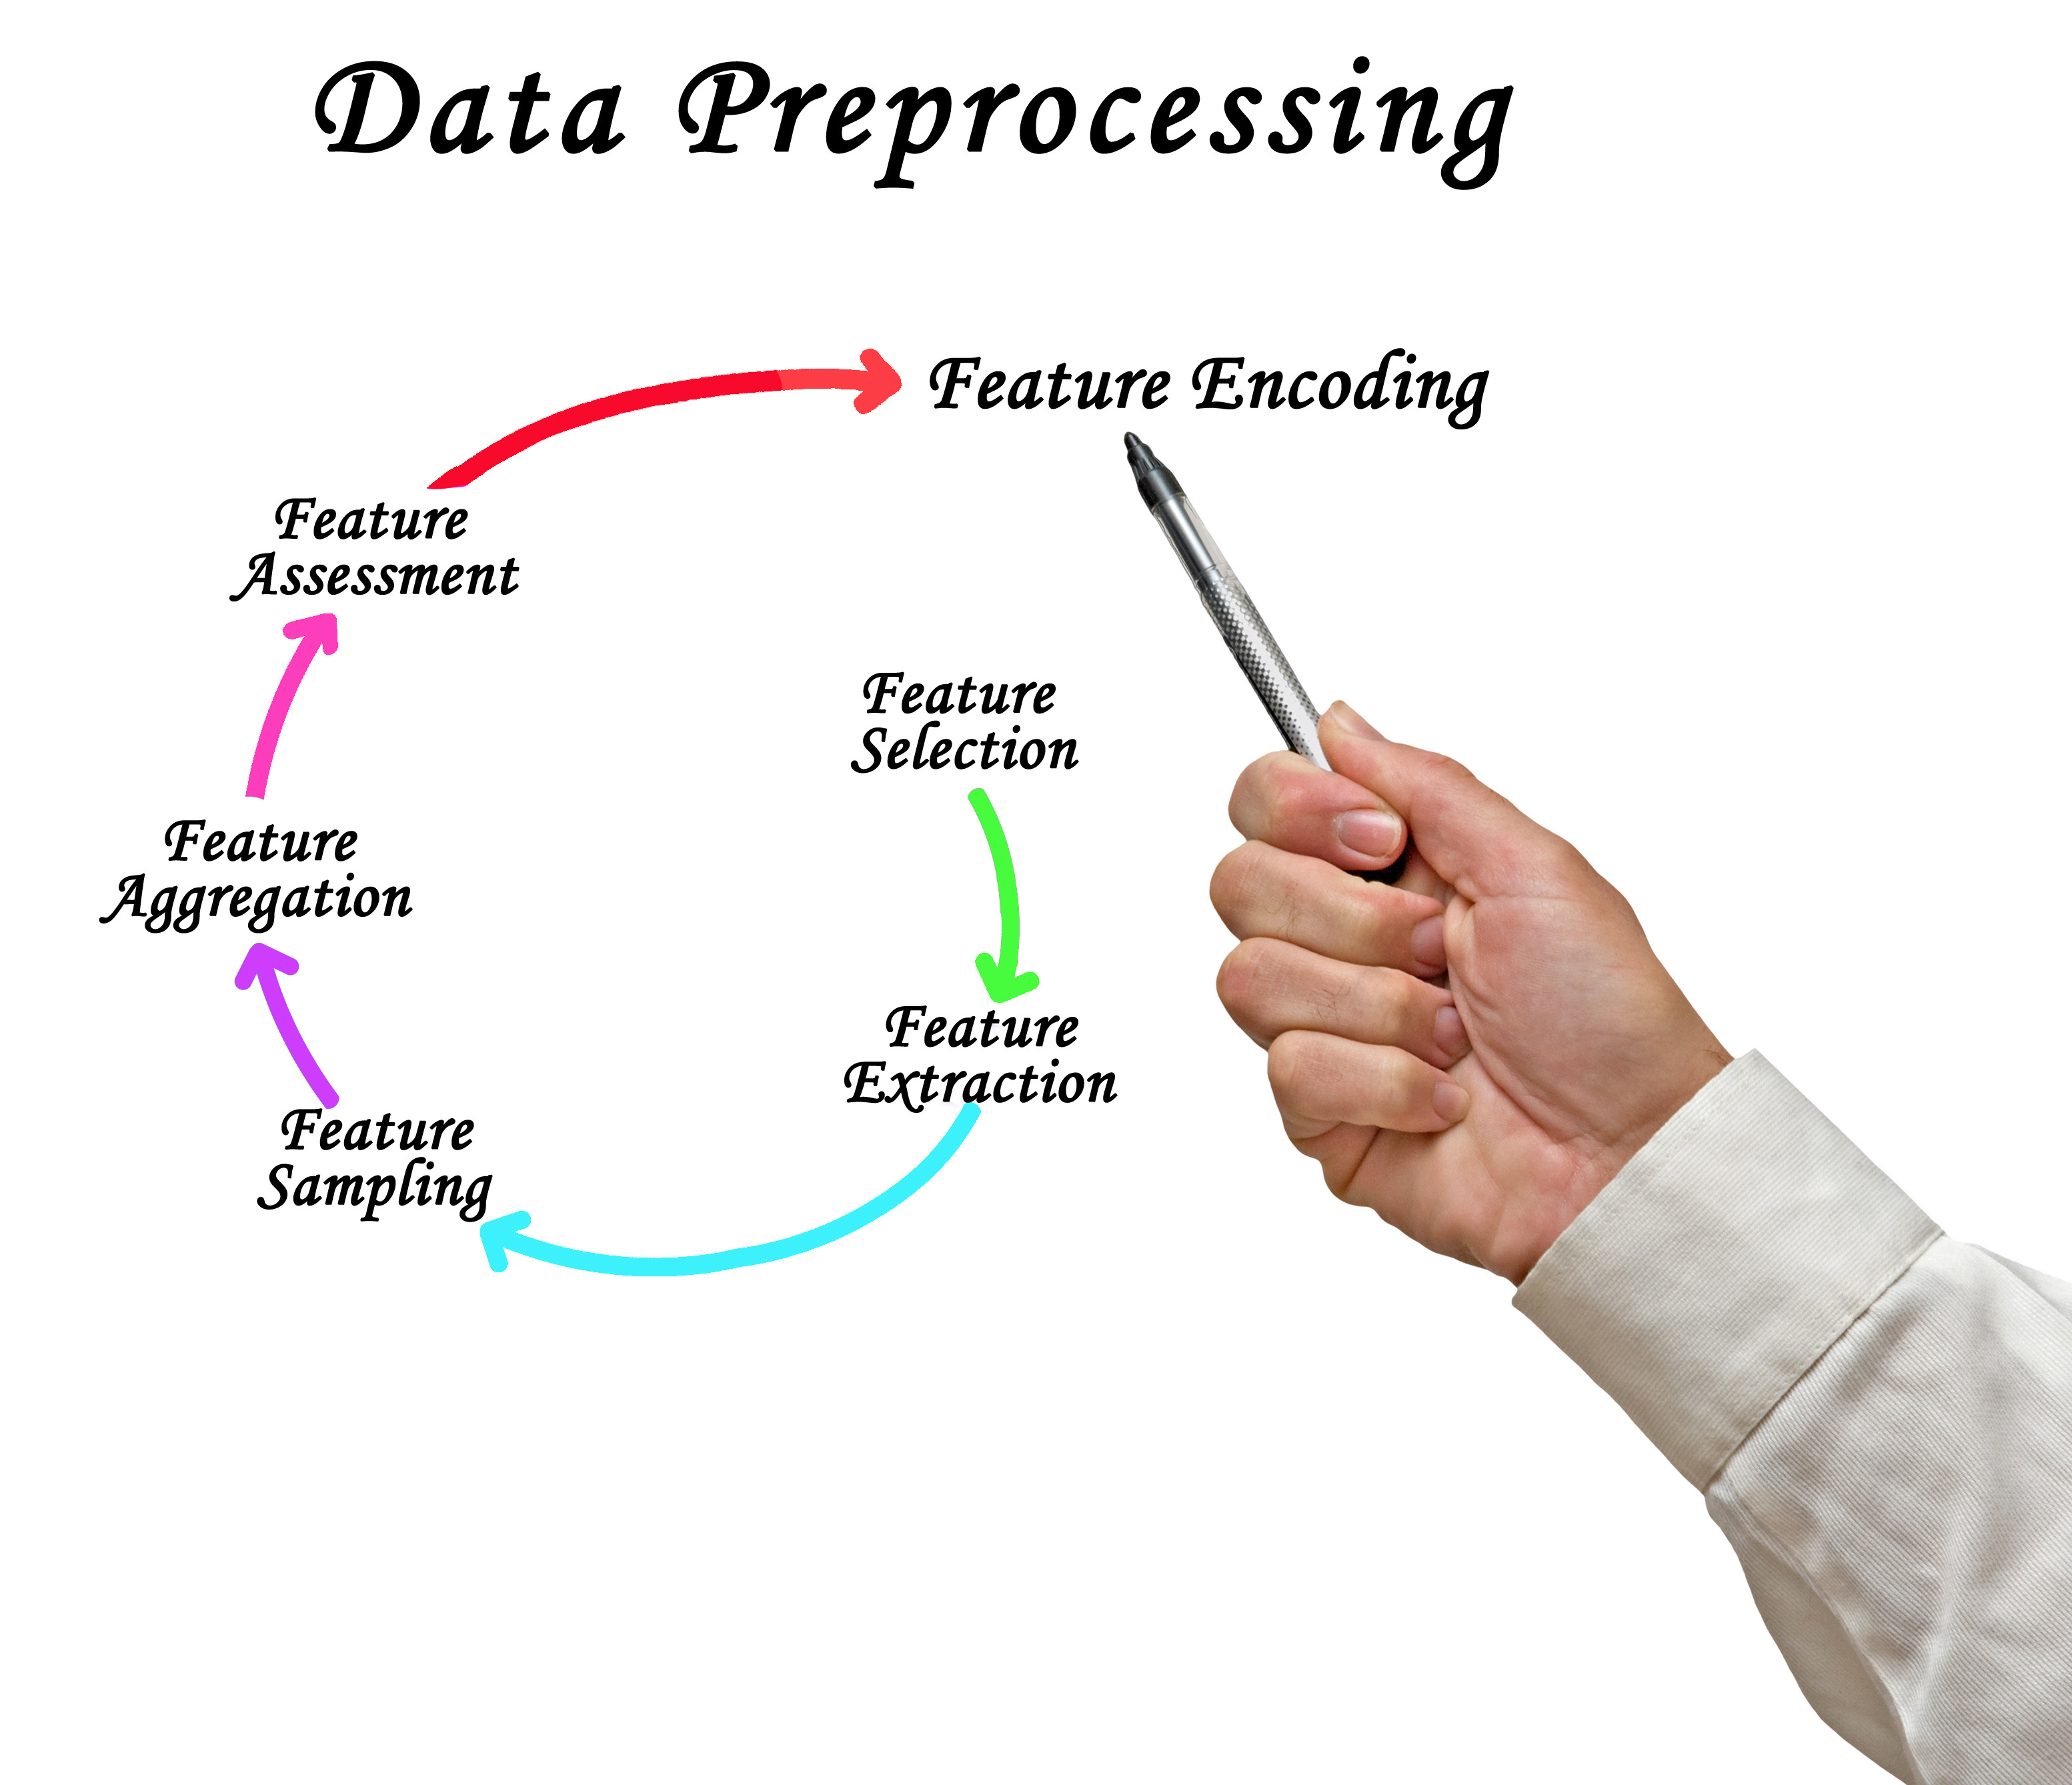
\includegraphics[keepaspectratio]{../../images/preprocess.jpeg}}
\end{center}
\end{column}

\begin{column}{0.6\linewidth}
O pré-processamento de dados inclui diversas atividades, como
\textbf{limpeza de dados}, \textbf{transformação de dados},
\textbf{redução de dimensão}, \textbf{seleção de recursos},
\textbf{normalização} e \textbf{amostragem}.
\end{column}
\end{columns}

👉 O \textbf{objetivo geral} do pré-processamento de dados é
\textbf{aumentar a qualidade} e a \textbf{precisão da análise} de dados,
\textbf{minimizando a influência de ruídos} e \textbf{inconsistências}
nos resultados finais.
\end{frame}

\begin{frame}{Importância do pré-processamento}
\phantomsection\label{importuxe2ncia-do-pruxe9-processamento}
O pré-processamento de dados é uma etapa importante e crítica no
processo de análise de dados. Algumas razões pelas quais é importante
realizar o pré-processamento são:

\pause

👉 \textbf{Melhoria da qualidade dos dados:} O pré-processamento de
dados pode ajudar a melhorar a qualidade dos dados, eliminando dados
duplicados, ausentes ou inconsistentes. Isso resulta em dados mais
precisos e confiáveis para análise.

\pause

👉 \textbf{Ajuste dos dados para a análise:} Muitos modelos e algoritmos
de análise de dados requerem que os dados estejam em um formato
específico. Na etapa do pré-processamento de dados ajusta-se os dados
para que estejam em um formato adequado para a análise.
\end{frame}

\begin{frame}{Importância do pré-processamento}
\phantomsection\label{importuxe2ncia-do-pruxe9-processamento-1}
👉 \textbf{Eliminação de ruídos:} Os dados geralmente contêm ruídos,
como outliers e valores extremos, que podem afetar negativamente a
precisão dos resultados finais. Nesta etapa, elimina-se esses ruídos,
tornando os resultados mais precisos.

\pause

👉 \textbf{Redução da complexidade dos dados:} Podemos reduzir a
complexidade dos dados, eliminando variáveis desnecessárias e reduzindo
o número de dimensões do conjunto de dados. Isso torna mais fácil a
análise e interpretação dos dados.

\pause

👉 \textbf{Melhoria do desempenho do modelo:} O pré-processamento de
dados pode ajudar a melhorar o desempenho do modelo, ao remover dados
redundantes, normalizar os dados e selecionar os recursos mais
importantes. Isso resulta em modelos mais precisos e confiáveis.
\end{frame}

\begin{frame}{Importância do pré-processamento}
\phantomsection\label{importuxe2ncia-do-pruxe9-processamento-2}
\begin{figure}[H]

{\centering \pandocbounded{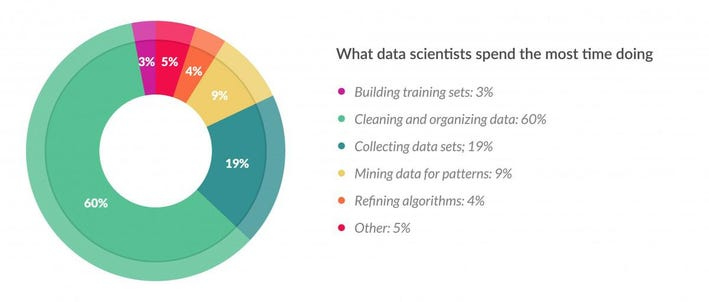
\includegraphics[keepaspectratio]{../../images/time.jpg}}

}

\caption{\href{https://www.forbes.com/sites/gilpress/2016/03/23/data-preparation-most-time-consuming-least-enjoyable-data-science-task-survey-says/?sh=34ce9abe6f63}{Fonte:
Forbes}}

\end{figure}%
\end{frame}

\begin{frame}{Importância do pré-processamento}
\phantomsection\label{importuxe2ncia-do-pruxe9-processamento-3}

\includegraphics[width=0.7\linewidth,height=\textheight,keepaspectratio]{../../images/impor_pre_process.png}
\end{frame}

\begin{frame}{O que há de errado nessa base?}
\phantomsection\label{o-que-huxe1-de-errado-nessa-base}
Usuário

Idade

Cidade

Data

Salário

Npáginas

Nsessões

Nprodutos

Clique

Comprou

user1

22

Belo Horizonte

22/10/21

1200

5

2

5

no

no

user2

1

São paulo

20/09/22

5000

21

4

11

yes

yes

user3

41

BH

23 de dezembro 2022

12000

2

1

3

NA

yes

user4

32

Miami

22/10/01

50000

NA

5

2

yes

no

user5

20

Tokyo

23/01/25

12220

5

5

8

no

yes

user6

28

NY

March 14, 2018

250000

8

NA

NA

no

yes
\end{frame}

\begin{frame}{Principais problemas com dados reais}
\phantomsection\label{principais-problemas-com-dados-reais}
\begin{center}
\pandocbounded{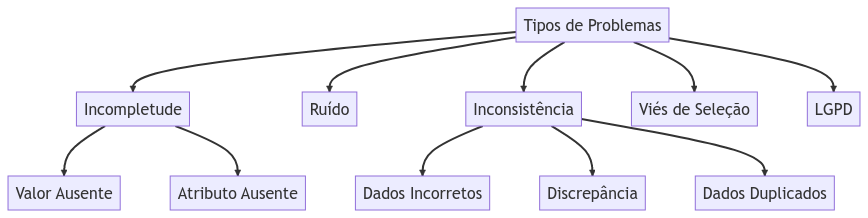
\includegraphics[keepaspectratio]{../../images/tipos.png}}
\end{center}
\end{frame}

\begin{frame}{Tipos de dados}
\phantomsection\label{tipos-de-dados}
Os dados podem ser classificados em três tipos principais:
\textbf{estruturados}, \textbf{semiestruturados} e \textbf{não
estruturados}

👉 \textbf{Estruturados}

São dados organizados em uma estrutura definida, como tabelas, colunas e
linhas em um banco de dados.

\begin{itemize}
\tightlist
\item
  \textbf{Exemplos:} informações de vendas, cadastros de clientes,
  registros de transações financeiras, entre outros.
\end{itemize}

\pause

💻 Para dados estruturados, a técnica de pré-processamento mais comum é
a \textbf{limpeza de dados}, além da \textbf{seleção de atributos
relevantes}, \textbf{normalização} e \textbf{transformação} de dados.
\end{frame}

\begin{frame}{Tipos de dados}
\phantomsection\label{tipos-de-dados-1}
👉 \textbf{Semiestruturados}

São dados que não possuem uma estrutura rígida como os dados
estruturados, mas possuem algumas formas de organização, como
marcadores, tags ou atributos.

\begin{itemize}
\tightlist
\item
  \textbf{Exemplos:} arquivos XML, JSON, HTML, entre outros.
\end{itemize}

\pause

💻 Para dados semiestruturados, a técnica de pré-processamento mais
comum é a \textbf{extração de informações relevantes}, que envolve a
identificação de padrões e estruturas em dados como XML, JSON ou HTML,
além da \textbf{extração de dados} a partir dessas estruturas.
\end{frame}

\begin{frame}{Tipos de dados}
\phantomsection\label{tipos-de-dados-2}
👉 \textbf{Não estruturados}

São dados que não possuem uma estrutura definida e estão em formato
livre, como texto, imagens, vídeos, áudios, e-mails, redes sociais,
entre outros.

\pause

💻 Exigem o uso de técnicas mais avançadas de \textbf{processamento de
linguagem natural}, \textbf{reconhecimento de padrões} e
\textbf{aprendizado de máquina}.

\pause

Com o aumento da quantidade de dados gerados diariamente, a análise de
\textbf{dados semiestruturados} e \textbf{não estruturados} tem se
tornado cada vez mais importante para empresas que desejam obter
insights valiosos sobre seus clientes, mercado e tendências.
\end{frame}

\begin{frame}{Processo de preparação da base de dados}
\phantomsection\label{processo-de-preparauxe7uxe3o-da-base-de-dados}
\begin{center}
\pandocbounded{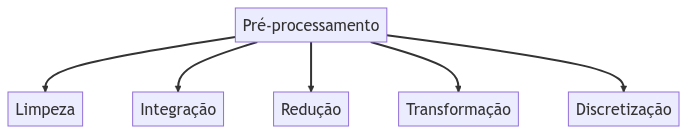
\includegraphics[keepaspectratio]{../../images/pre.png}}
\end{center}
\end{frame}

\begin{frame}{Limpeza de dados}
\phantomsection\label{limpeza-de-dados}
🤔 O que é limpeza de dados? 🧹

\begin{itemize}
\tightlist
\item
  \textbf{Limpeza de dados} é o processo de \textbf{identificar},
  \textbf{remover} ou \textbf{corrigir dados imprecisos},
  \textbf{incompletos}, \textbf{inconsistentes}, \textbf{duplicados} ou
  \textbf{irrelevantes} em um conjunto de dados.
\end{itemize}

\pause

\begin{itemize}
\tightlist
\item
  É uma etapa \textbf{importante} no processo de análise de dados, uma
  vez que \textbf{dados sujos} podem \textbf{afetar negativamente} a
  \textbf{qualidade} e \textbf{confiabilidade} dos resultados da
  análise.
\end{itemize}
\end{frame}

\begin{frame}{Identificação de problemas}
\phantomsection\label{identificauxe7uxe3o-de-problemas}
👉 Existem várias técnicas para identificar problemas de limpeza de
dados em um conjunto de dados. Algumas das técnicas mais comuns incluem:

\begin{itemize}
\tightlist
\item
  \textbf{Análise visual:} pode-se inspecionar o conjunto de dados para
  identificar erros óbvios, como valores ausentes, valores que não fazem
  sentido ou valores extremos.
\end{itemize}

\begin{figure}[H]

{\centering \pandocbounded{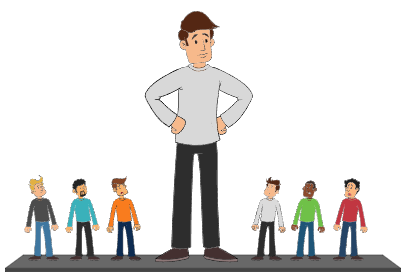
\includegraphics[keepaspectratio]{../../images/outlier.png}}

}

\caption{\href{https://www.nagwa.com/en/explainers/845148137695/}{Fonte:Nagwa}}

\end{figure}%
\end{frame}

\begin{frame}{Identificação de problemas}
\phantomsection\label{identificauxe7uxe3o-de-problemas-1}
\begin{itemize}
\tightlist
\item
  \textbf{Estatística descritiva:} realizar uma boa análise descritiva.
  Valores extremos ou valores que estão muito longe do intervalo
  interquartil, por exemplo, podem ser indicativos de problemas de
  limpeza de dados.
\end{itemize}

\begin{figure}[H]

{\centering \pandocbounded{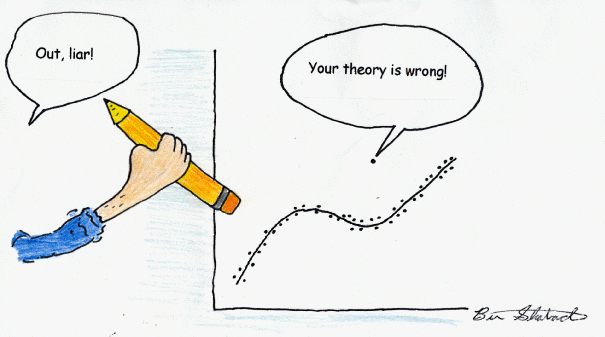
\includegraphics[keepaspectratio]{../../images/outlier2.png}}

}

\caption{\href{https://davidmlane.com/ben/cartoons.html}{Fonte:Statistics
Cartoons by Ben Shabad}}

\end{figure}%
\end{frame}

\begin{frame}{Identificação de problemas}
\phantomsection\label{identificauxe7uxe3o-de-problemas-2}
\begin{itemize}
\tightlist
\item
  \textbf{Gráficos de distribuição:} analisar os gráficos de
  distribuição para cada variável e observar padrões incomuns na
  distribuição dos valores, como bimodalidade, assimetria ou outliers.
\end{itemize}

\begin{center}
\pandocbounded{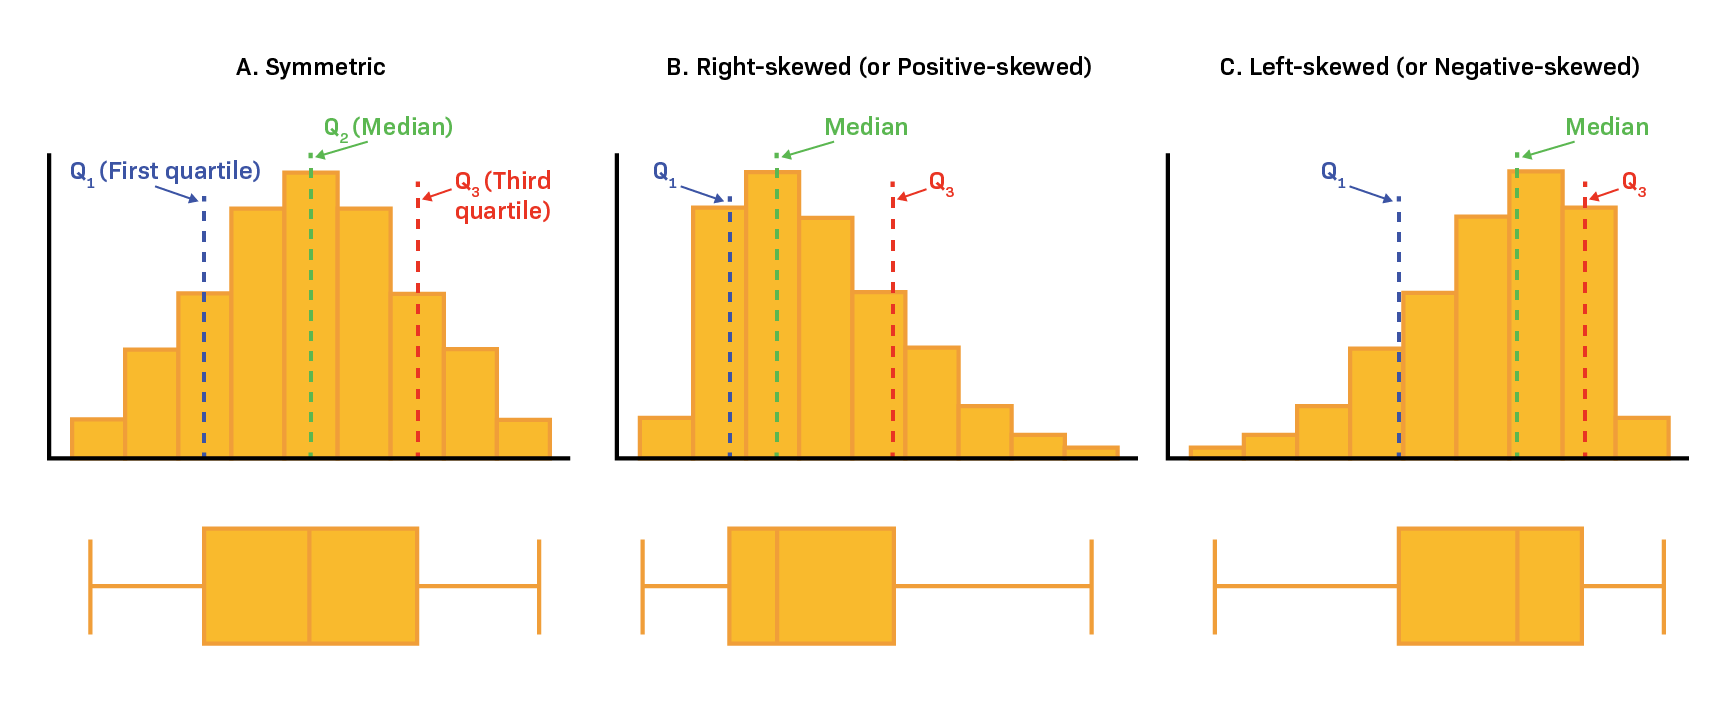
\includegraphics[keepaspectratio]{../../images/assimetrica.png}}
\end{center}
\end{frame}

\begin{frame}{Identificação de problemas}
\phantomsection\label{identificauxe7uxe3o-de-problemas-3}
\begin{itemize}
\tightlist
\item
  \textbf{Análise de correlação:} analisar as correlações entre as
  variáveis e procurar relações que não fazem sentido ou que não
  deveriam existir.
\end{itemize}

\begin{figure}[H]

{\centering \pandocbounded{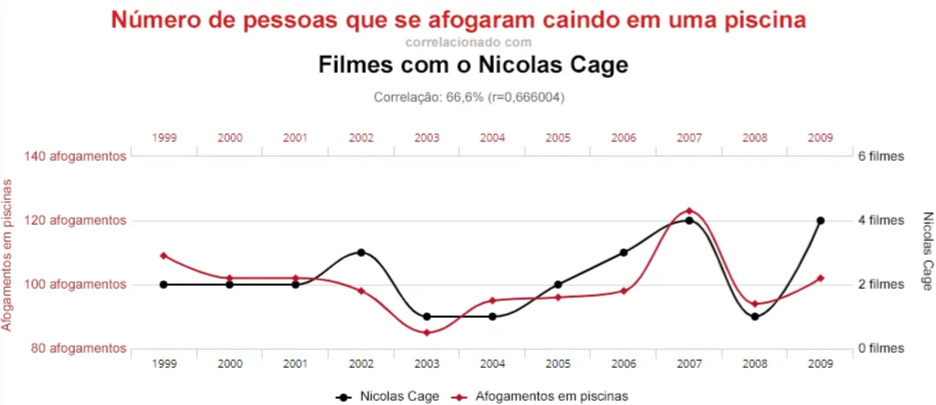
\includegraphics[keepaspectratio]{../../images/espurias.png}}

}

\caption{\href{https://euleralencar.medium.com/o-que-é-a-correlação-espúria-819b77482764}{Fonte:Medium}}

\end{figure}%
\end{frame}

\begin{frame}{Identificação de problemas}
\phantomsection\label{identificauxe7uxe3o-de-problemas-4}
\begin{itemize}
\tightlist
\item
  \textbf{Análise de consistência:} comparar valores em diferentes
  variáveis para ver se eles são consistentes entre si.

  \begin{itemize}
  \tightlist
  \item
    Por exemplo, se uma pessoa é descrita como tendo 2 metros de altura
    e 30 kg de peso, pode haver um problema de limpeza de dados.
  \end{itemize}
\end{itemize}

\begin{center}
\pandocbounded{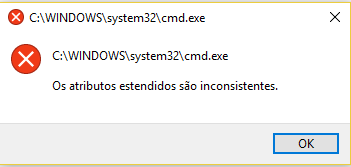
\includegraphics[keepaspectratio]{../../images/inconsistentes.png}}
\end{center}
\end{frame}

\begin{frame}{Tratamento de dados faltantes}
\phantomsection\label{tratamento-de-dados-faltantes}

\includegraphics[width=0.7\linewidth,height=\textheight,keepaspectratio]{../../images/missing.png}
\end{frame}

\begin{frame}{Tratamento de dados faltantes}
\phantomsection\label{tratamento-de-dados-faltantes-1}
\begin{columns}[T]
\begin{column}{0.5\linewidth}
\begin{quote}
``The idea of imputation is both seductive and dangerous''.
\end{quote}

Madow et al. (1983)
\end{column}

\begin{column}{0.5\linewidth}
\begin{center}
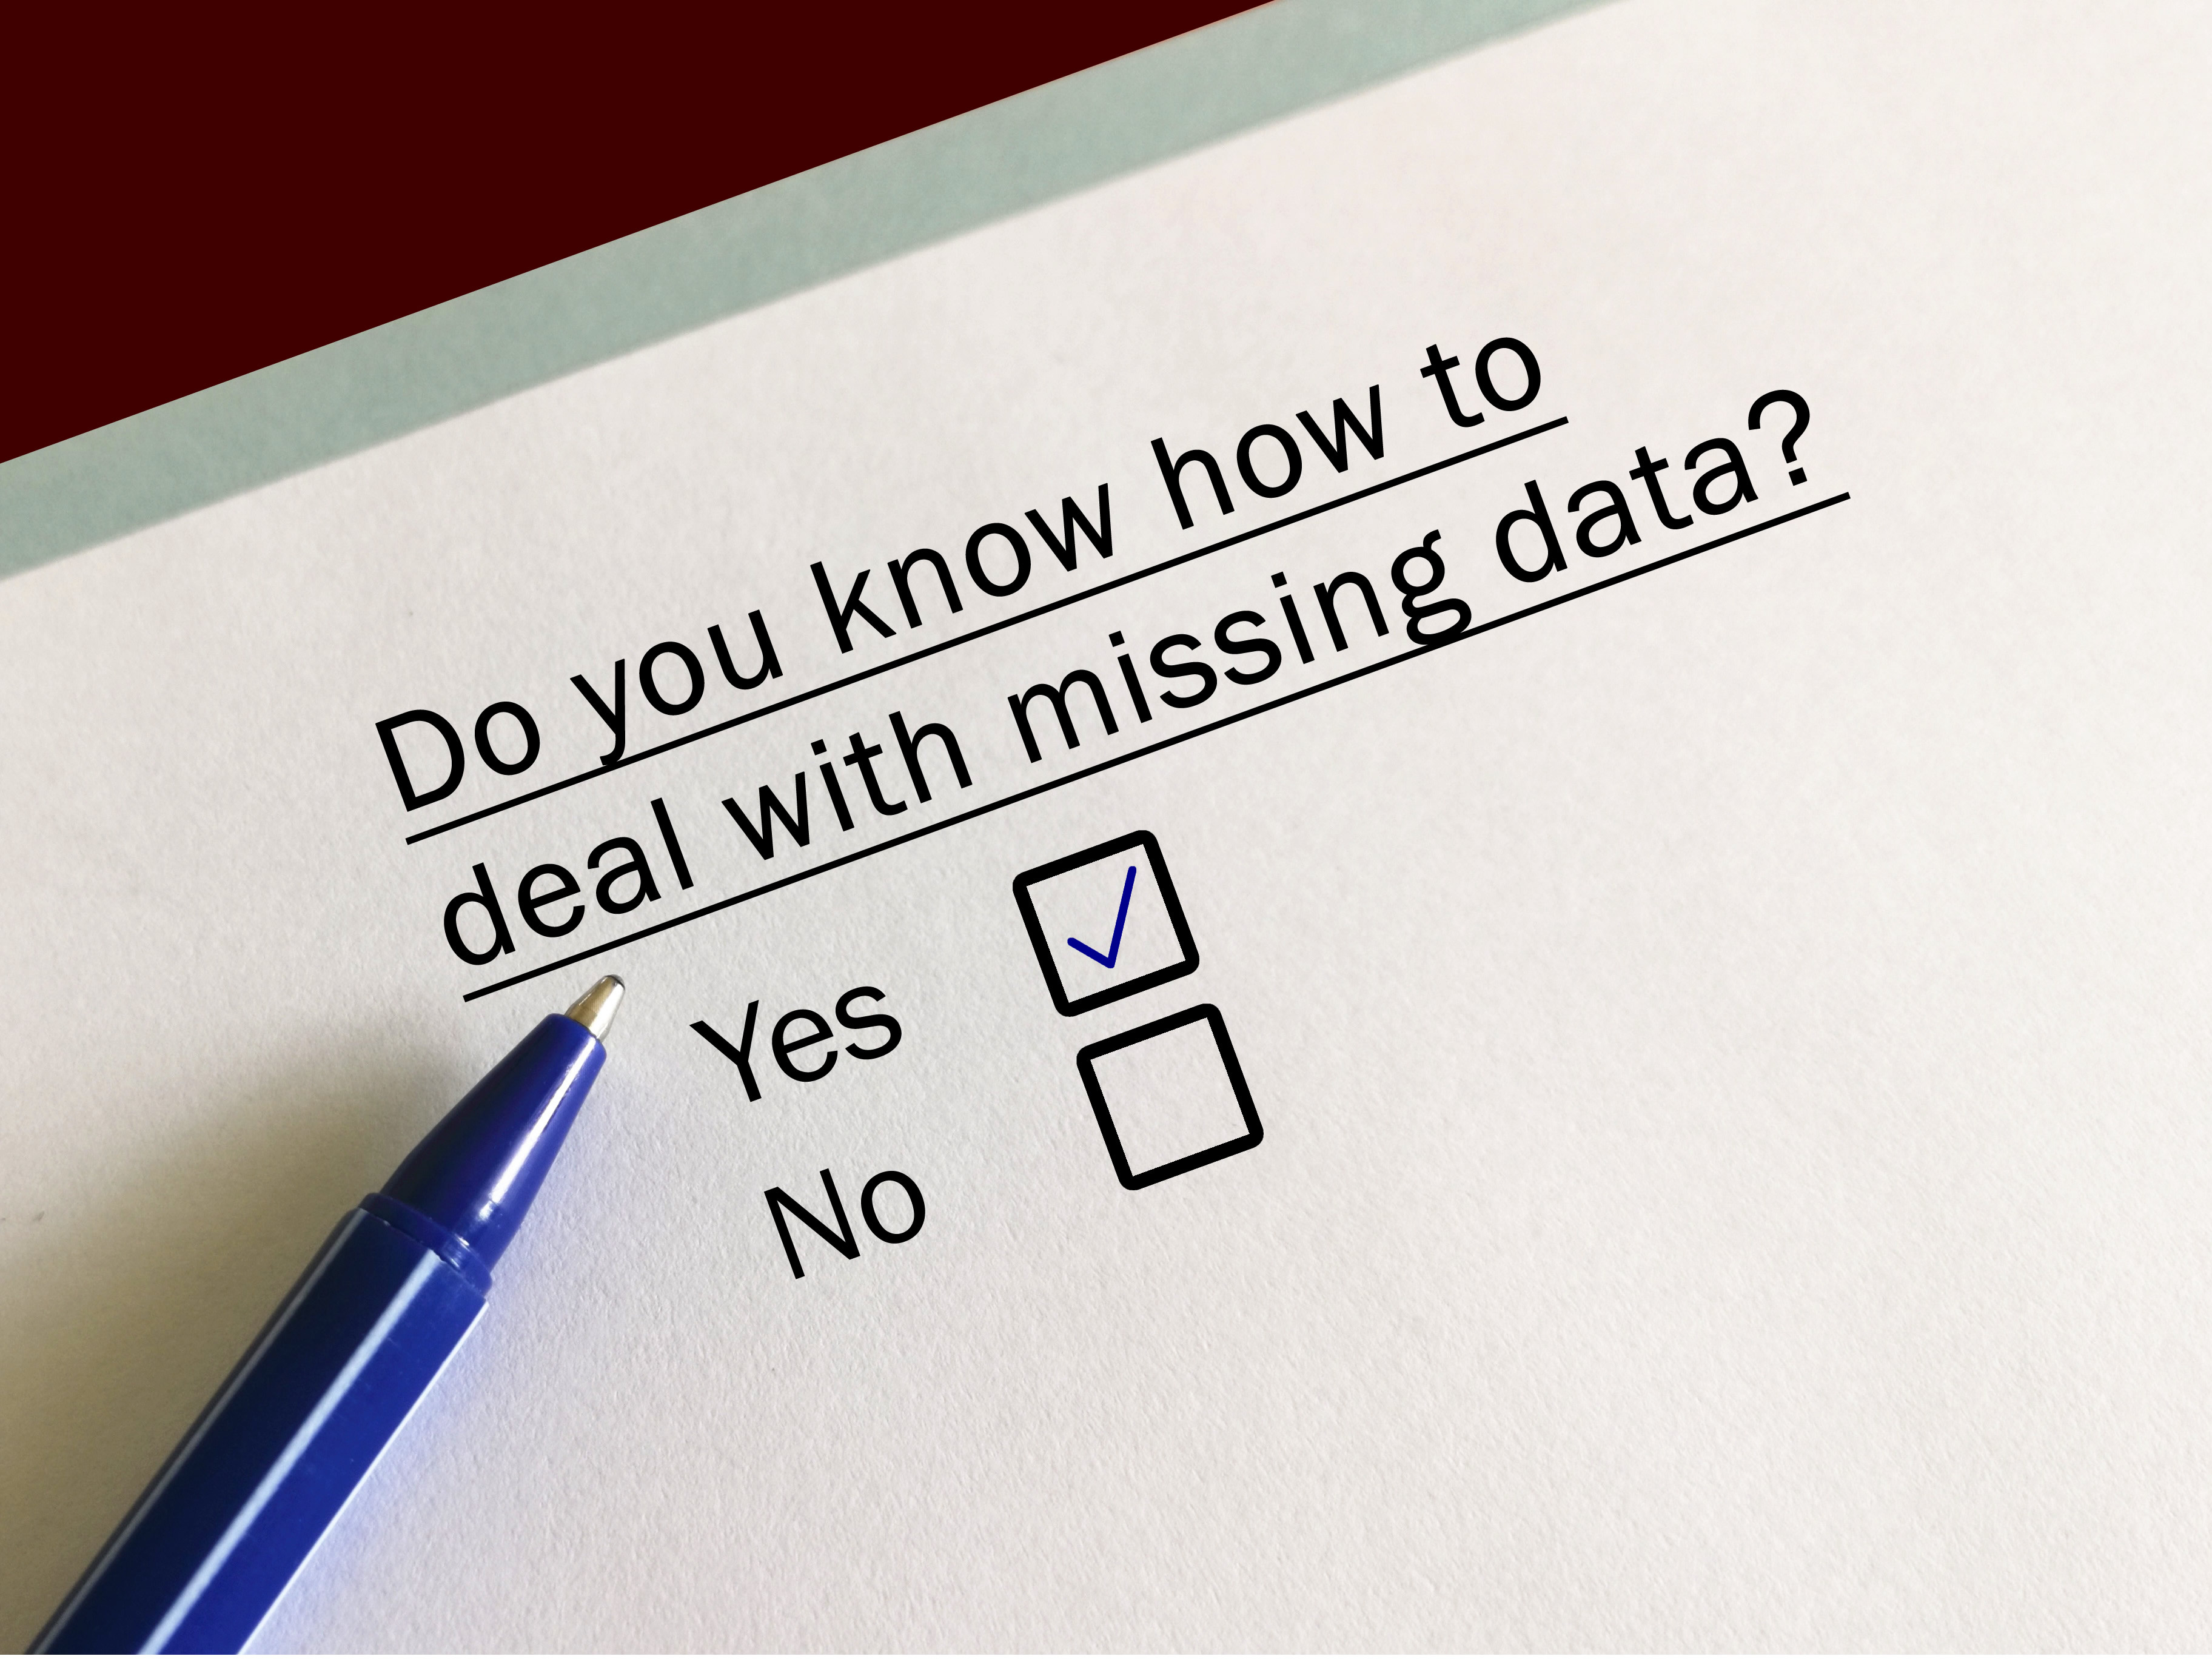
\includegraphics[width=7.29167in,height=\textheight,keepaspectratio]{../../images/missing.jpeg}
\end{center}
\end{column}
\end{columns}

A escolha do método de tratamento de valor ausente \textbf{depende do
tipo de valor ausente} identificado. Basicamente, existem dois tipos de
valores ausentes: \textbf{aleatórios} e \textbf{não aleatórios}
\end{frame}

\begin{frame}{Mecanismo gerador dos dados faltantes}
\phantomsection\label{mecanismo-gerador-dos-dados-faltantes}
\begin{columns}[T]
\begin{column}{0.5\linewidth}
\begin{center}
\includegraphics[width=4.16667in,height=\textheight,keepaspectratio]{../../images/dice.png}
\end{center}
\end{column}

\begin{column}{0.5\linewidth}
\textbf{MCAR (missing completely at random):} ocorrem de forma
\textbf{completamente aleatória} e \textbf{não estão relacionados} com
as outras variáveis do conjunto de dados.
\end{column}
\end{columns}

👉 Por exemplo, em uma pesquisa por telefone algumas das respostas não
foram registradas devido a problemas técnicos que ocorreram
aleatoriamente durante a coleta dos dados.
\end{frame}

\begin{frame}{Mecanismo gerador dos dados faltantes}
\phantomsection\label{mecanismo-gerador-dos-dados-faltantes-1}
\begin{columns}[T]
\begin{column}{0.5\linewidth}
\textbf{MNAR (missing not at random):} são valores ausentes que
\textbf{estão relacionados} com outras variáveis do conjunto de dados e
podem levar a \textbf{enviesamento} na análise dos dados.
\end{column}

\begin{column}{0.5\linewidth}
\begin{center}
\includegraphics[width=7.29167in,height=\textheight,keepaspectratio]{../../images/not_randon.jpeg}
\end{center}
\end{column}
\end{columns}

👉 Por exemplo, em uma pesquisa sobre saúde mental, as pessoas que
sofrem de depressão tendem a não responder perguntas sobre sua condição
de saúde mental.
\end{frame}

\begin{frame}{Como identificar o mecanismo gerador dos dados faltantes?}
\phantomsection\label{como-identificar-o-mecanismo-gerador-dos-dados-faltantes}
\begin{columns}[T]
\begin{column}{0.5\linewidth}
\begin{center}
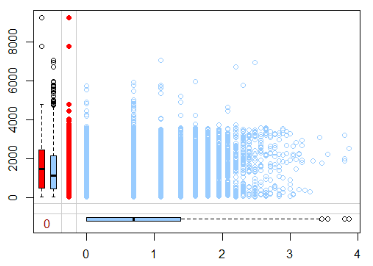
\includegraphics[width=6.25in,height=\textheight,keepaspectratio]{../../images/margin_plot.png}
\end{center}
\end{column}

\begin{column}{0.5\linewidth}
Para identificar \textbf{valores ausentes MCAR}, uma técnica é analisar
a \textbf{distribuição de valores ausentes} em relação às \textbf{outras
variáveis} do conjunto de dados.
\end{column}
\end{columns}

👉 Se \textbf{não houver correlação} entre a \textbf{ausência de
valores} e outras variáveis, é provável que os valores ausentes
\textbf{sejam MCAR}.
\end{frame}

\begin{frame}{Como identificar o mecanismo gerador dos dados faltantes?}
\phantomsection\label{como-identificar-o-mecanismo-gerador-dos-dados-faltantes-1}
👉 Também é possível realizar testes estatísticos para verificar se a
distribuição dos valores ausentes é aleatória ou não.

\pause

🙁 Já a identificação de \textbf{valores ausentes MNAR} é mais complexa,
pois eles estão relacionados a outras variáveis do conjunto de dados e,
portanto, é mais difícil determinar se eles são \textbf{completamente
aleatórios} ou \textbf{não}.
\end{frame}

\begin{frame}{Como identificar o mecanismo gerador dos dados faltantes?}
\phantomsection\label{como-identificar-o-mecanismo-gerador-dos-dados-faltantes-2}
👉 Algumas técnicas para identificar valores ausentes MNAR incluem:

\pause

\begin{itemize}
\tightlist
\item
  \textbf{Análise de padrões de resposta:} é possível analisar como
  objetos com valores ausentes se diferenciam daqueles que não têm
  valores ausentes, em termos dos atributos.
\end{itemize}

\begin{columns}[T]
\begin{column}{0.5\linewidth}
\begin{center}
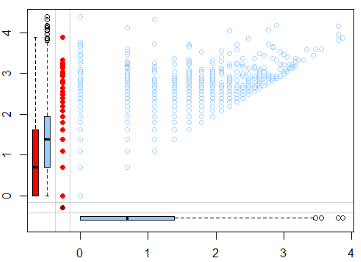
\includegraphics[width=6.25in,height=\textheight,keepaspectratio]{../../images/margin_plot_2.png}
\end{center}
\end{column}

\begin{column}{0.5\linewidth}
Se os indivíduos com \textbf{valores ausentes} são
\textbf{significativamente diferentes} em relação a essas variáveis, é
provável que os \textbf{valores ausentes sejam MNAR}.
\end{column}
\end{columns}
\end{frame}

\begin{frame}{Como identificar o mecanismo gerador dos dados faltantes?}
\phantomsection\label{como-identificar-o-mecanismo-gerador-dos-dados-faltantes-3}
\begin{itemize}
\tightlist
\item
  \textbf{Análise de correlação:} é possível analisar a correlação entre
  as variáveis com valores ausentes e outras variáveis no conjunto de
  dados.

  \begin{itemize}
  \tightlist
  \item
    Se houver uma correlação significativa entre as variáveis, é
    possível que os valores ausentes sejam MNAR.
  \end{itemize}
\end{itemize}
\end{frame}

\begin{frame}{Como identificar o mecanismo gerador dos dados faltantes?}
\phantomsection\label{como-identificar-o-mecanismo-gerador-dos-dados-faltantes-4}
\begin{itemize}
\item
  \textbf{Análise visual:} é possível realizar análises gráficas para
  verificar se há algum padrão de valores ausentes que sugira que eles
  não são aleatórios.

  \begin{itemize}
  \tightlist
  \item
    Por exemplo, pode-se criar um gráfico de dispersão de uma variável
    em relação a outra, marcando as observações com valores ausentes. Se
    houver um padrão na localização dos valores ausentes no gráfico, é
    possível que eles sejam MNAR.
  \end{itemize}
\end{itemize}
\end{frame}

\begin{frame}{Tratamento de valores ausentes completamente aleatórios}
\phantomsection\label{tratamento-de-valores-ausentes-completamente-aleatuxf3rios}
O tratamento de \textbf{valores ausentes completamente aleatórios
(MCAR)} é relativamente simples, pois os valores ausentes são
\textbf{independentes} das demais variáveis e podem ser tratados
\textbf{sem viés}.
\end{frame}

\begin{frame}{Tratamento de valores ausentes completamente aleatórios}
\phantomsection\label{tratamento-de-valores-ausentes-completamente-aleatuxf3rios-1}
\begin{columns}[T]
\begin{column}{0.5\linewidth}
\textbf{Exclusão de registros com valores ausentes:} Se a proporção de
valores ausentes é pequena em relação ao tamanho do conjunto de dados, é
possível excluir os registros que contêm valores ausentes sem
comprometer a análise.
\end{column}

\begin{column}{0.5\linewidth}
\begin{center}

\includegraphics[width=6.25in,height=\textheight,keepaspectratio]{../../images/delete.jpeg}
\end{center}
\end{column}
\end{columns}

No entanto, isso pode levar a uma \textbf{perda de informações valiosas}
e \textbf{reduzir o tamanho} do conjunto de dados.
\end{frame}

\begin{frame}{Tratamento de valores ausentes completamente aleatórios}
\phantomsection\label{tratamento-de-valores-ausentes-completamente-aleatuxf3rios-2}
\begin{columns}[T]
\begin{column}{0.5\linewidth}
\textbf{Imputação de valores:} Se o número de valores ausentes é grande,
é possível imputar os valores ausentes usando métodos estatísticos, como
a média, mediana ou regressão.
\end{column}

\begin{column}{0.5\linewidth}
\begin{center}
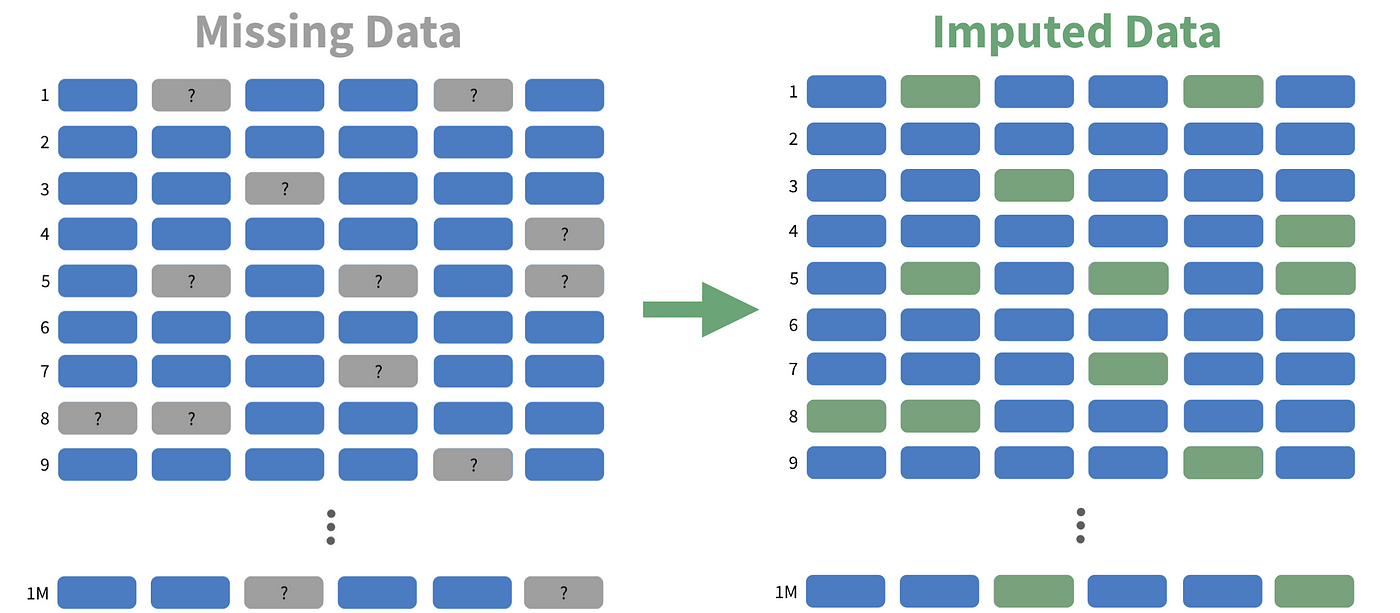
\includegraphics[width=6.25in,height=\textheight,keepaspectratio]{../../images/imputacao.png}
\end{center}
\end{column}
\end{columns}

Esses métodos são \textbf{simples} e \textbf{rápidos}, mas podem
\textbf{introduzir um viés nos resultados}, dependendo da
\textbf{distribuição dos valores ausentes} e da escolha do método de
imputação.
\end{frame}

\begin{frame}{Tratamento de valores ausentes completamente aleatórios}
\phantomsection\label{tratamento-de-valores-ausentes-completamente-aleatuxf3rios-3}
\begin{columns}[T]
\begin{column}{0.5\linewidth}
\begin{center}
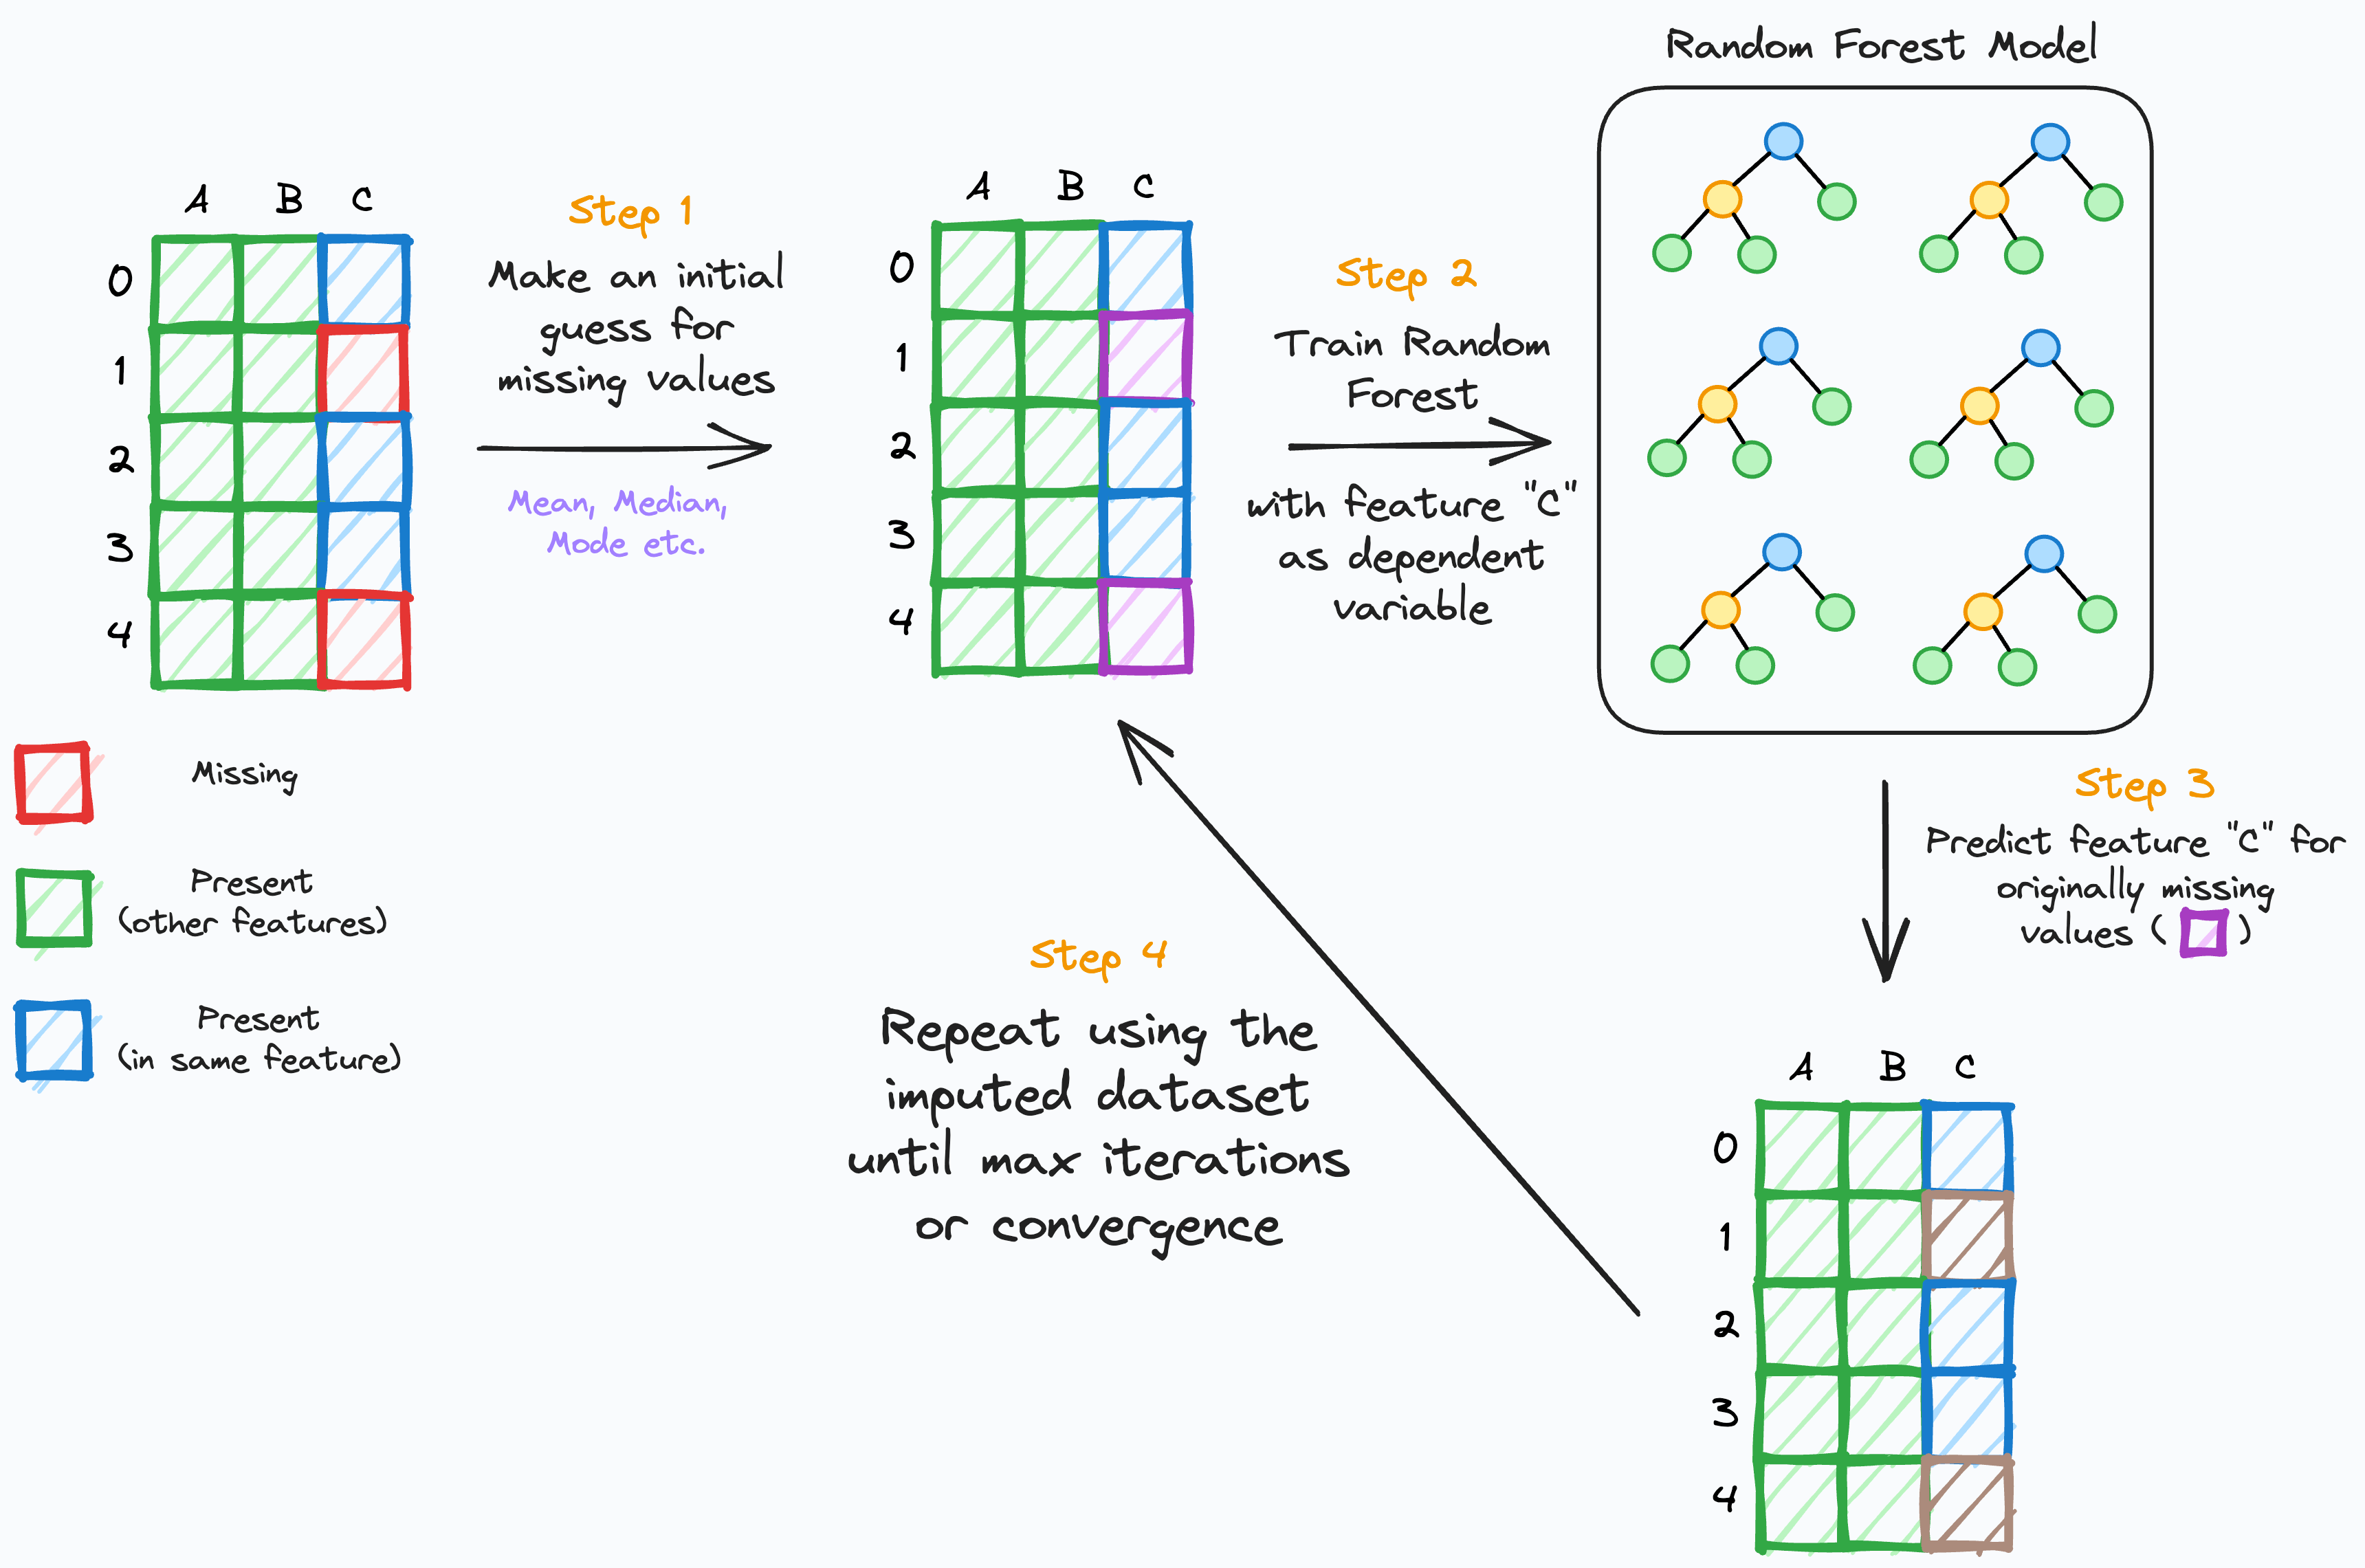
\includegraphics[width=6.25in,height=\textheight,keepaspectratio]{../../images/imput_ML.png}
\end{center}
\end{column}

\begin{column}{0.5\linewidth}
\textbf{Modelagem com técnicas de aprendizado de máquina:} As técnicas
de aprendizado de máquina podem ajudar a prever valores ausentes com
base em outros dados disponíveis.
\end{column}
\end{columns}

\textbf{Mais precisa} do que a imputação de valores, mas também pode ser
\textbf{mais complexa} e exigir um \textbf{conjunto de dados de
treinamento grande} o suficiente para o \textbf{modelo aprender a
relação entre as variáveis}.
\end{frame}

\begin{frame}{Tratamento de valores ausentes não aleatórios}
\phantomsection\label{tratamento-de-valores-ausentes-nuxe3o-aleatuxf3rios}
O tratamento de \textbf{valores ausentes não aleatórios (MNAR)} é
\textbf{mais complexo} do que o tratamento de \textbf{valores ausentes
completamente aleatórios (MCAR)}, pois os valores ausentes estão
\textbf{relacionados} a outras variáveis do conjunto de dados e podem
levar a um \textbf{viés na análise} se não forem tratados adequadamente.
\end{frame}

\begin{frame}{Tratamento de valores ausentes não aleatórios}
\phantomsection\label{tratamento-de-valores-ausentes-nuxe3o-aleatuxf3rios-1}
\begin{itemize}
\tightlist
\item
  \textbf{Modelagem com técnicas de aprendizado de máquina:} Como os
  valores ausentes MNAR estão relacionados a outras variáveis do
  conjunto de dados, a modelagem com técnicas de aprendizado de máquina
  pode ser uma abordagem útil para prever os valores ausentes com base
  nas informações disponíveis.
\end{itemize}

\pause

\begin{itemize}
\item
  \textbf{Imputação baseada em modelos:} A imputação baseada em modelos
  é uma técnica que envolve a construção de um modelo estatístico para
  prever os valores ausentes com base nas informações disponíveis.

  \begin{itemize}
  \tightlist
  \item
    Essa abordagem requer um conhecimento prévio da relação entre as
    variáveis e pode ser mais complexa do que outros métodos de
    imputação.
  \end{itemize}
\end{itemize}
\end{frame}

\begin{frame}{Tratamento de valores ausentes não aleatórios}
\phantomsection\label{tratamento-de-valores-ausentes-nuxe3o-aleatuxf3rios-2}
\begin{itemize}
\item
  \textbf{Análise de sensibilidade:} A análise de sensibilidade é uma
  técnica que envolve testar diferentes cenários e valores de imputação
  para avaliar o impacto nos resultados da análise.

  \begin{itemize}
  \tightlist
  \item
    Essa abordagem pode ajudar a identificar os valores mais plausíveis
    para a imputação e a avaliar a robustez dos resultados.
  \end{itemize}
\end{itemize}
\end{frame}

\begin{frame}{Tratamento de valores ausentes não aleatórios}
\phantomsection\label{tratamento-de-valores-ausentes-nuxe3o-aleatuxf3rios-3}
Uma vez que os valores ausentes estão \textbf{relacionados} a outras
variáveis do conjunto de dados, há um \textbf{padrão de ausência}
definido em MNAR, que pode ser importante.

\begin{columns}[T]
\begin{column}{0.5\linewidth}
Uma maneira de \textbf{reter esse padrão de ausência} é adicionando uma
\textbf{variável binária}, indicando se a \textbf{característica foi
imputada}.
\end{column}

\begin{column}{0.5\linewidth}
\begin{center}
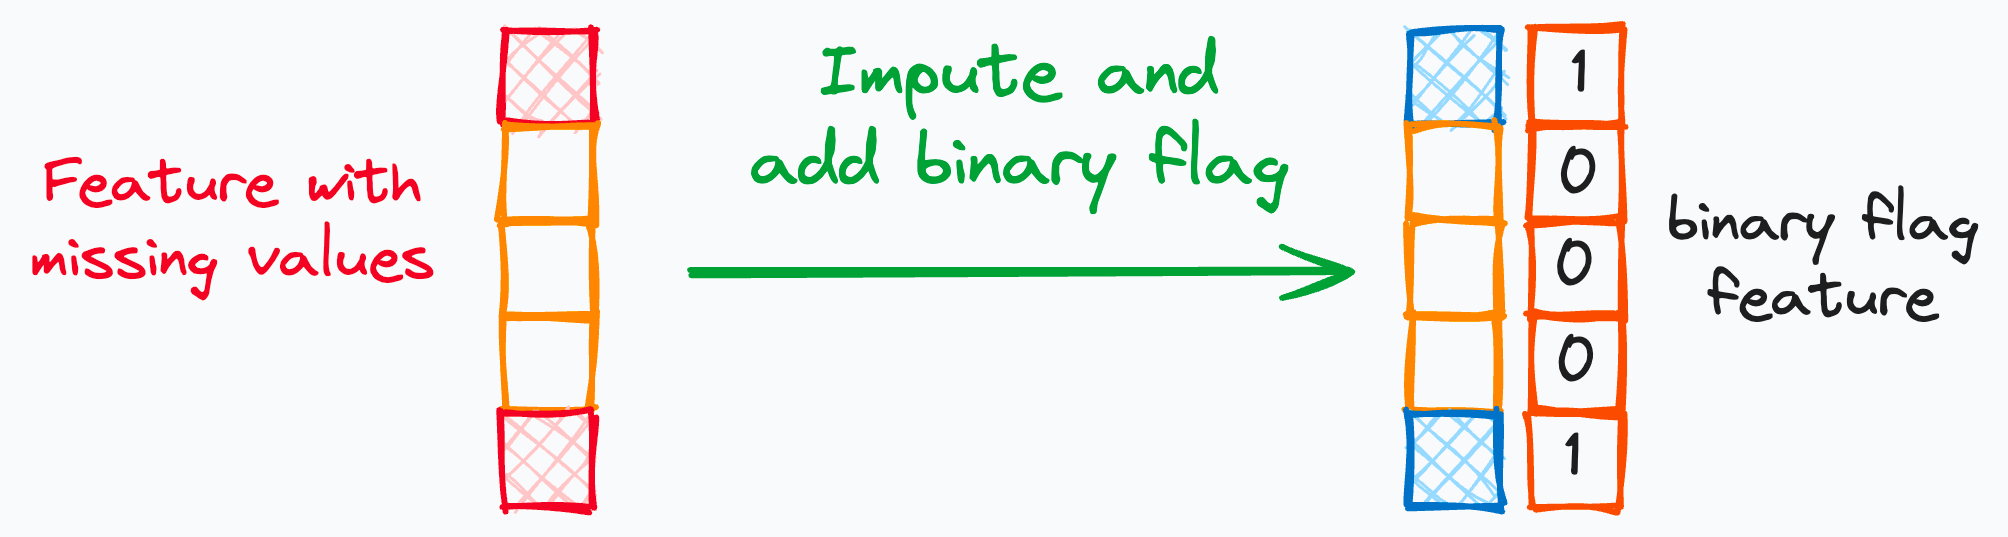
\includegraphics[width=8.33333in,height=\textheight,keepaspectratio]{../../images/imput_bin.png}
\end{center}
\end{column}
\end{columns}
\end{frame}

\begin{frame}{Tratamento de valores inconsistentes}
\phantomsection\label{tratamento-de-valores-inconsistentes}
O tratamento de valores inconsistentes é importante para garantir a
qualidade e a confiabilidade dos dados {→} podem afetar negativamente a
análise e a interpretação dos resultados.

\begin{center}
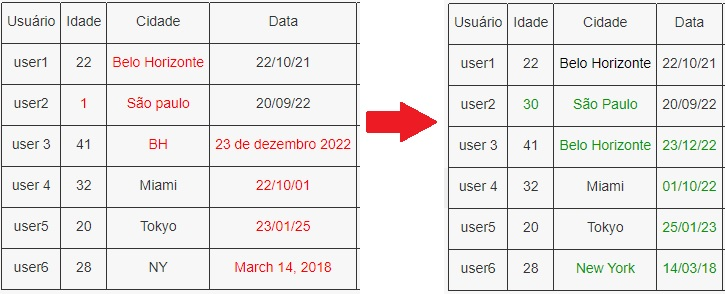
\includegraphics[width=6.25in,height=\textheight,keepaspectratio]{../../images/inconsistente.jpg}
\end{center}
\end{frame}

\begin{frame}{Tratamento de valores inconsistentes}
\phantomsection\label{tratamento-de-valores-inconsistentes-1}
Algumas técnicas comuns para lidar com valores inconsistentes incluem:

\begin{itemize}
\tightlist
\item
  \textbf{Identificação de valores inconsistentes:} Verifica-se os
  valores em cada variável, comparando-os com os valores esperados ou
  com outras fontes de dados. Também é possível usar técnicas de
  detecção de outliers para identificar valores inconsistentes
  automaticamente.
\end{itemize}

\pause

\begin{itemize}
\item
  \textbf{Correção manual:} Para valores inconsistentes que podem ser
  facilmente corrigidos, a correção manual pode ser uma abordagem
  eficaz.

  \begin{itemize}
  \tightlist
  \item
    Isso pode incluir a revisão manual dos dados e a correção de erros,
    como erros de digitação ou valores fora do intervalo esperado.
  \end{itemize}
\end{itemize}
\end{frame}

\begin{frame}{Tratamento de valores inconsistentes}
\phantomsection\label{tratamento-de-valores-inconsistentes-2}
\begin{itemize}
\item
  \textbf{Imputação de valores:} Para valores inconsistentes que não
  podem ser facilmente corrigidos, a imputação de valores pode ser uma
  abordagem útil.

  \begin{itemize}
  \tightlist
  \item
    Isso envolve a substituição de valores inconsistentes por valores
    estimados com base em outras informações disponíveis no conjunto de
    dados.
  \end{itemize}
\end{itemize}

\pause

\begin{itemize}
\item
  \textbf{Exclusão de registros:} Para valores inconsistentes que não
  podem ser corrigidos e não podem ser imputados com precisão, a
  exclusão de registros pode ser uma abordagem apropriada.

  \begin{itemize}
  \tightlist
  \item
    Isso envolve a remoção dos registros com valores inconsistentes do
    conjunto de dados.
  \end{itemize}
\end{itemize}
\end{frame}

\begin{frame}{Tratamento de ruídos}
\phantomsection\label{tratamento-de-ruuxeddos}

\includegraphics[width=0.7\linewidth,height=\textheight,keepaspectratio]{../../images/ruidosos.png}
\end{frame}

\begin{frame}{Tratamento de ruídos}
\phantomsection\label{tratamento-de-ruuxeddos-1}
\textbf{Ruído}, no contexto da \textbf{estatística e análise de dados},
refere-se a qualquer tipo de \textbf{interferência} ou
\textbf{distorção} que pode obscurecer ou alterar a interpretação dos
dados coletados.

\pause

Esse fenômeno pode surgir de \textbf{diversas fontes}, como erros de
entrada de dados, erros de medição, valores atípicos, variabilidade
aleatória ou viés e influências externas que \textbf{não estão
diretamente relacionadas ao fenômeno em estudo}.

\pause

O ruído pode ser considerado um \textbf{fator indesejado} que compromete
a \textbf{precisão} e a \textbf{confiabilidade} das análises
estatísticas.
\end{frame}

\begin{frame}{Tratamento de ruídos}
\phantomsection\label{tratamento-de-ruuxeddos-2}
\begin{center}

\includegraphics[width=0.9\linewidth,height=\textheight,keepaspectratio]{pre_processamento_files/figure-beamer/unnamed-chunk-1-1.png}
\end{center}
\end{frame}

\begin{frame}{Tratamento de ruídos}
\phantomsection\label{tratamento-de-ruuxeddos-3}
\begin{itemize}
\tightlist
\item
  O \textbf{sinal} contém a estrutura que queremos aprender\\
\item
  O \textbf{ruído} dificulta a identificação dessa estrutura\\
\item
  Um modelo ruim pode confundir ruído com padrão
\end{itemize}

\begin{tcolorbox}[enhanced jigsaw, rightrule=.15mm, bottomrule=.15mm, colframe=quarto-callout-important-color-frame, breakable, left=2mm, colback=white, arc=.35mm, toprule=.15mm, leftrule=.75mm, opacityback=0]
\begin{minipage}[t]{5.5mm}
\textcolor{quarto-callout-important-color}{\faExclamation}
\end{minipage}%
\begin{minipage}[t]{\textwidth - 5.5mm}

\textbf{Overfitting ocorre quando o modelo aprende o ruído em vez do
sinal.}

\end{minipage}%
\end{tcolorbox}
\end{frame}

\begin{frame}{Tratamento de ruídos}
\phantomsection\label{tratamento-de-ruuxeddos-4}
Como lidar com variações indesejadas nos dados?

\begin{tcolorbox}[enhanced jigsaw, rightrule=.15mm, bottomrule=.15mm, colframe=quarto-callout-important-color-frame, breakable, left=2mm, colback=white, arc=.35mm, toprule=.15mm, leftrule=.75mm, opacityback=0]
\begin{minipage}[t]{5.5mm}
\textcolor{quarto-callout-important-color}{\faExclamation}
\end{minipage}%
\begin{minipage}[t]{\textwidth - 5.5mm}

O objetivo não é eliminar o ruído, mas reduzir seu impacto sem perder o
sinal.

\end{minipage}%
\end{tcolorbox}

\begin{itemize}
\tightlist
\item
  Limpeza de dados\\
\item
  Transformações\\
\item
  Suavização\\
\item
  Modelagem robusta
\end{itemize}
\end{frame}

\begin{frame}{Tratamento de ruídos}
\phantomsection\label{tratamento-de-ruuxeddos-5}
\begin{block}{Valores atípicos (outliers)}
\phantomsection\label{valores-atuxedpicos-outliers}
Valores muito distantes do padrão dos dados
\end{block}

\begin{columns}[T]
\begin{column}{0.5\linewidth}
\begin{block}{❌ Remover}
\phantomsection\label{remover}
Quando:

\begin{itemize}
\tightlist
\item
  erro de medição\\
\item
  erro de digitação\\
\item
  valor impossível
\end{itemize}

👉 Ex: idade = 250
\end{block}
\end{column}

\begin{column}{0.5\linewidth}
\begin{block}{⚠️ Manter}
\phantomsection\label{manter}
Quando:

\begin{itemize}
\tightlist
\item
  observação real\\
\item
  evento raro importante\\
\item
  comportamento relevante
\end{itemize}

👉 Ex: cliente que gasta muito
\end{block}
\end{column}
\end{columns}
\end{frame}

\begin{frame}
\begin{columns}[T]
\begin{column}{0.5\linewidth}
\begin{block}{🔧 Transformar}
\phantomsection\label{transformar}
\begin{itemize}
\tightlist
\item
  log, raiz, Box-Cox\\
\item
  reduz impacto extremo
\end{itemize}
\end{block}
\end{column}

\begin{column}{0.5\linewidth}
\begin{block}{🤖 Modelar de forma robusta}
\phantomsection\label{modelar-de-forma-robusta}
\begin{itemize}
\tightlist
\item
  regressão robusta, árvores de decisão, random forest

  \begin{itemize}
  \tightlist
  \item
    menos sensíveis a outliers
  \end{itemize}
\end{itemize}
\end{block}
\end{column}
\end{columns}

\begin{tcolorbox}[enhanced jigsaw, rightrule=.15mm, opacitybacktitle=0.6, left=2mm, colback=white, titlerule=0mm, coltitle=black, bottomtitle=1mm, colframe=quarto-callout-important-color-frame, breakable, arc=.35mm, toptitle=1mm, toprule=.15mm, bottomrule=.15mm, title=\textcolor{quarto-callout-important-color}{\faExclamation}\hspace{0.5em}{Importante}, opacityback=0, leftrule=.75mm, colbacktitle=quarto-callout-important-color!10!white]

A decisão depende do contexto do problema.

\end{tcolorbox}
\end{frame}

\begin{frame}
\begin{block}{Como identificar valores atípicos?}
\phantomsection\label{como-identificar-valores-atuxedpicos}
\begin{columns}[T]
\begin{column}{0.5\linewidth}
\begin{block}{📊 Métodos estatísticos}
\phantomsection\label{muxe9todos-estatuxedsticos}
\begin{itemize}
\tightlist
\item
  \textbf{Boxplot}\\
\item
  \textbf{Z-score}

  \begin{itemize}
  \tightlist
  \item
    \textbar z\textbar{} \textgreater{} 3 → possível outlier
  \end{itemize}
\item
  \textbf{\(IQR:\)} \(Q_3 - Q_1\)

  \begin{itemize}
  \tightlist
  \item
    \(< Q_1 − 1,5 \times IQR\)\\
  \item
    \(> Q_3 + 1,5 \times IQR\)
  \end{itemize}
\end{itemize}
\end{block}
\end{column}

\begin{column}{0.5\linewidth}
\begin{block}{🤖 Métodos baseados em dados}
\phantomsection\label{muxe9todos-baseados-em-dados}
\begin{itemize}
\tightlist
\item
  \textbf{DBSCAN}

  \begin{itemize}
  \tightlist
  \item
    identifica pontos isolados\\
  \item
    fora de clusters
  \end{itemize}
\end{itemize}

👉 útil em dados complexos
\end{block}
\end{column}
\end{columns}

\begin{tcolorbox}[enhanced jigsaw, rightrule=.15mm, bottomrule=.15mm, colframe=quarto-callout-warning-color-frame, breakable, left=2mm, colback=white, arc=.35mm, toprule=.15mm, leftrule=.75mm, opacityback=0]
\begin{minipage}[t]{5.5mm}
\textcolor{quarto-callout-warning-color}{\faExclamationTriangle}
\end{minipage}%
\begin{minipage}[t]{\textwidth - 5.5mm}

Valores atípicos podem ser \textbf{erro} ou \textbf{informação
relevante}.

\end{minipage}%
\end{tcolorbox}

\begin{tcolorbox}[enhanced jigsaw, rightrule=.15mm, bottomrule=.15mm, colframe=quarto-callout-tip-color-frame, breakable, left=2mm, colback=white, arc=.35mm, toprule=.15mm, leftrule=.75mm, opacityback=0]
\begin{minipage}[t]{5.5mm}
\textcolor{quarto-callout-tip-color}{\faLightbulb}
\end{minipage}%
\begin{minipage}[t]{\textwidth - 5.5mm}

Documente sempre as decisões de tratamento de dados.

\end{minipage}%
\end{tcolorbox}
\end{block}
\end{frame}

\begin{frame}{Tratamento de ruídos}
\phantomsection\label{tratamento-de-ruuxeddos-6}
\begin{block}{Suavização de dados}
\phantomsection\label{suavizauxe7uxe3o-de-dados}
Reduz variações aleatórias mantendo o padrão

\begin{itemize}
\tightlist
\item
  Média móvel\\
\item
  LOESS\\
\item
  Suavização exponencial
\end{itemize}

\begin{tcolorbox}[enhanced jigsaw, rightrule=.15mm, opacitybacktitle=0.6, left=2mm, colback=white, titlerule=0mm, coltitle=black, bottomtitle=1mm, colframe=quarto-callout-important-color-frame, breakable, arc=.35mm, toptitle=1mm, toprule=.15mm, bottomrule=.15mm, title=\textcolor{quarto-callout-important-color}{\faExclamation}\hspace{0.5em}{Importante}, opacityback=0, leftrule=.75mm, colbacktitle=quarto-callout-important-color!10!white]

Suavizar não remove dados: revela o comportamento subjacente.

\end{tcolorbox}
\end{block}
\end{frame}

\begin{frame}
\begin{center}

\includegraphics[width=0.9\linewidth,height=\textheight,keepaspectratio]{pre_processamento_files/figure-beamer/unnamed-chunk-2-1.png}
\end{center}
\end{frame}

\begin{frame}{Integração de dados}
\phantomsection\label{integrauxe7uxe3o-de-dados}
\begin{columns}[T]
\begin{column}{0.5\linewidth}
\textbf{Integração de dados} é o processo de \textbf{combinar dados de
múltiplas fontes} em um \textbf{único conjunto de dados}
\textbf{coerente} e \textbf{integrado}.
\end{column}

\begin{column}{0.5\linewidth}
\begin{center}
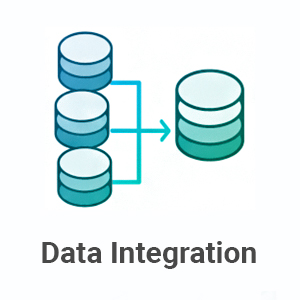
\includegraphics[width=5.20833in,height=\textheight,keepaspectratio]{../../images/Data-Integration.jpg}
\end{center}
\end{column}
\end{columns}

O \textbf{objetivo da integração de dados} é criar um conjunto de dados
mais \textbf{completo} e \textbf{preciso}, permitindo análises mais
\textbf{abrangentes} e \textbf{informadas}.
\end{frame}

\begin{frame}{Integração de dados}
\phantomsection\label{integrauxe7uxe3o-de-dados-1}
\begin{itemize}
\item
  \textbf{Fusão de dados:} é o processo de combinar dois ou mais
  conjuntos de dados com base em uma chave comum.

  \begin{itemize}
  \tightlist
  \item
    Por exemplo, dados de clientes de uma empresa podem ser fundidos com
    dados de vendas, com base no número de identificação de cliente.
  \end{itemize}
\end{itemize}

\pause

\begin{itemize}
\item
  \textbf{Análise de correspondência:} é uma técnica de integração de
  dados que permite combinar informações de diferentes fontes, com base
  em uma análise de correspondência de variáveis.

  \begin{itemize}
  \tightlist
  \item
    Por exemplo, dados de vendas de uma empresa podem ser combinados com
    dados demográficos, com base em correspondências de variáveis, como
    localização geográfica ou faixa etária.
  \end{itemize}
\end{itemize}
\end{frame}

\begin{frame}{Integração de dados}
\phantomsection\label{integrauxe7uxe3o-de-dados-2}

{💡} Independentemente da técnica usada, é importante lembrar que a
\textbf{integração de dados} pode ser \textbf{complexa} e
\textbf{demorada} e pode envolver a \textbf{identificação} e
\textbf{correção de inconsistências nos dados}.
\end{frame}

\begin{frame}{Redução de dados}
\phantomsection\label{reduuxe7uxe3o-de-dados}
{💡} A \textbf{redução de dados} é uma técnica usada para
\textbf{diminuir a dimensão} de um conjunto de dados, ou seja, reduzir o
número de variáveis ou características que compõem o conjunto de dados.
\end{frame}

\begin{frame}{Redução de dados}
\phantomsection\label{reduuxe7uxe3o-de-dados-1}
\begin{itemize}
\item
  Existem várias razões para reduzir os dados:

  \begin{itemize}
  \tightlist
  \item
    \textbf{Simplificar} a análise de dados, tornando-a mais fácil e
    mais rápida de ser executada;
  \item
    \textbf{Reduzir} o tempo de processamento e armazenamento dos dados;
  \item
    \textbf{Melhorar} a qualidade dos dados, eliminando variáveis
    irrelevantes ou redundantes que possam afetar negativamente a
    análise;
  \item
    \textbf{Preparar} os dados para a entrada em um modelo de
    aprendizado de máquina.
  \end{itemize}
\end{itemize}
\end{frame}

\begin{frame}{Análise de Componentes Principais}
\phantomsection\label{anuxe1lise-de-componentes-principais}
\begin{center}
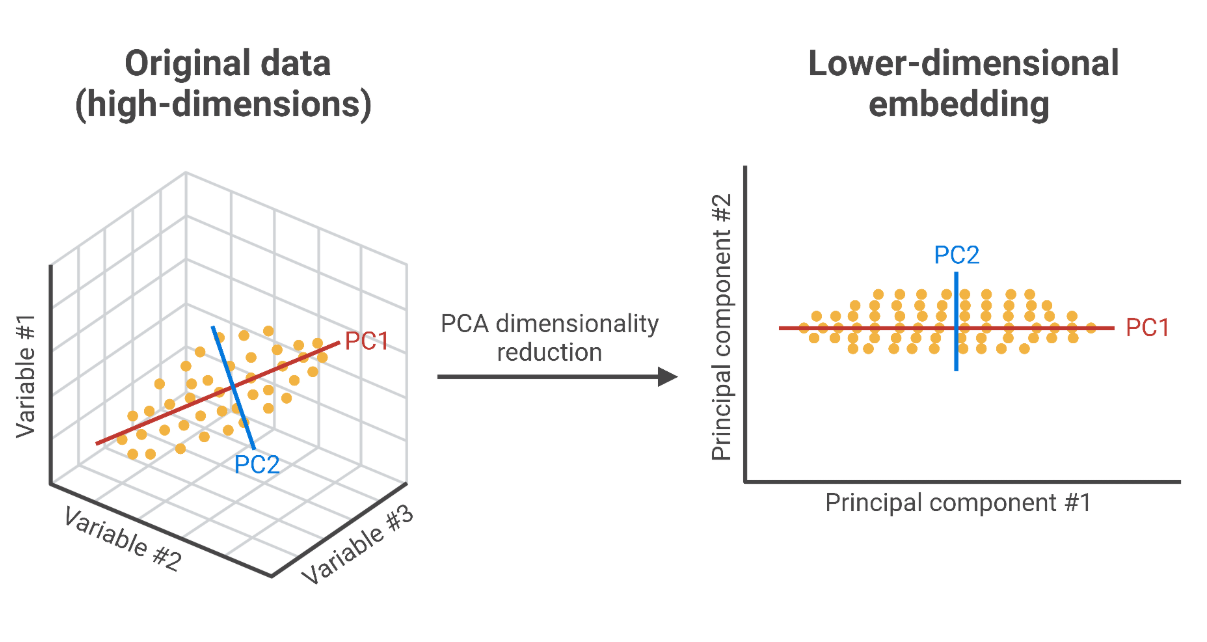
\includegraphics[width=5.20833in,height=\textheight,keepaspectratio]{../../images/pca.png}
\end{center}
\end{frame}

\begin{frame}{Amostragem}
\phantomsection\label{amostragem}
\begin{center}
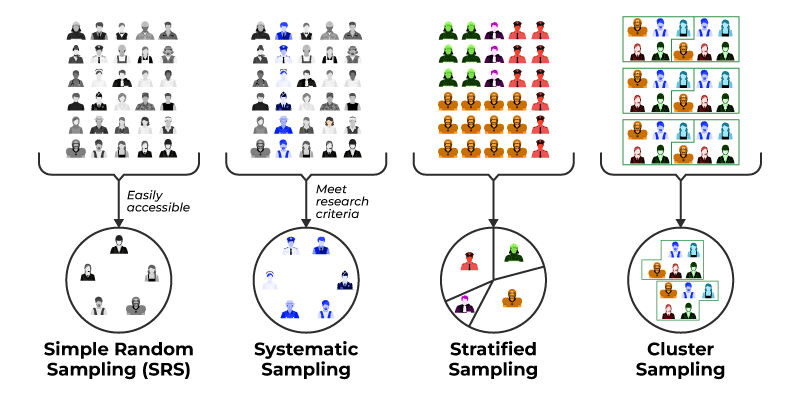
\includegraphics[width=5.20833in,height=\textheight,keepaspectratio]{../../images/sampling.png}
\end{center}
\end{frame}

\begin{frame}{Seleção de atributos}
\phantomsection\label{seleuxe7uxe3o-de-atributos}
\begin{itemize}
\tightlist
\item
  \textbf{Seleção de atributos} é um processo de pré-processamento de
  dados que envolve a \textbf{escolha dos atributos} (variáveis)
  \textbf{mais relevantes} para a análise.
\end{itemize}

\pause

\begin{itemize}
\tightlist
\item
  O objetivo da seleção de atributos é \textbf{reduzir a
  dimensionalidade dos dados}, eliminando características
  \textbf{irrelevantes} e \textbf{redundantes}, e, assim, melhorar a
  \textbf{precisão} e a \textbf{eficiência} da análise.
\end{itemize}
\end{frame}

\begin{frame}{Seleção de atributos}
\phantomsection\label{seleuxe7uxe3o-de-atributos-1}
\textbf{Seleção baseada em filtro:} Essa técnica usa métricas
estatísticas para avaliar a relevância dos atributos e seleciona aqueles
que têm maior correlação com a variável de interesse.

\begin{itemize}
\tightlist
\item
  \textbf{Métodos de filtragem:} coeficiente de correlação, ganho de
  informação e o teste de qui-quadrado.
\end{itemize}

\pandocbounded{
\includegraphics[keepaspectratio]{../../images/fig01.png}}
\end{frame}

\begin{frame}{Seleção de atributos}
\phantomsection\label{seleuxe7uxe3o-de-atributos-2}
\textbf{Seleção baseada em wrapper:} Essa técnica envolve a seleção de
atributos por meio de um modelo de aprendizado de máquina, que é
treinado em um conjunto de atributos selecionados. O modelo é avaliado
usando validação cruzada e as atributos são selecionados com base no
desempenho do modelo.

\begin{itemize}
\tightlist
\item
  \textbf{Métodos wrapper:} Forward stepwise selection, Backward
  Elimination.
\end{itemize}

\pandocbounded{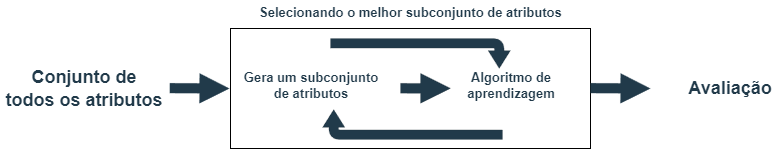
\includegraphics[keepaspectratio]{../../images/fig02.png}}
\end{frame}

\begin{frame}{Seleção de atributos}
\phantomsection\label{seleuxe7uxe3o-de-atributos-3}
\textbf{Seleção baseada em incorporação:} Essa técnica envolve a seleção
de atributos durante o processo de treinamento do modelo de aprendizado
de máquina. O modelo é treinado com todas os atributos e, em seguida, os
atributos são removidos com base em sua importância para o modelo.

\begin{itemize}
\tightlist
\item
  \textbf{Métodos de incorporação:} Regressão LASSO, Árvores de
  decisão\ldots{}
\end{itemize}

\pandocbounded{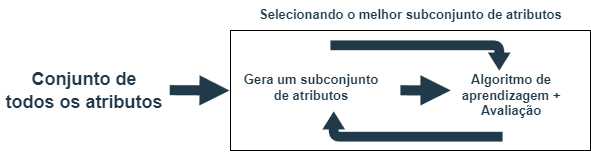
\includegraphics[keepaspectratio]{../../images/fig03.png}}
\end{frame}

\begin{frame}{Transformação de dados}
\phantomsection\label{transformauxe7uxe3o-de-dados}

\includegraphics[width=0.7\linewidth,height=\textheight,keepaspectratio]{../../images/fusion.png}
\end{frame}

\begin{frame}{Transformação de dados}
\phantomsection\label{transformauxe7uxe3o-de-dados-1}
As bases de dados brutas e integradas a partir de \textbf{bases
distintas} podem sofrer, além de \textbf{valores ausentes},
\textbf{ruídos} e \textbf{inconsistências}, de dados não ou pouco
\textbf{padronizados}.

\pause

\begin{itemize}
\tightlist
\item
  Por exemplo, pode haver valores de um mesmo atributo escritos em
  maiúsculo e outros em minúsculo, e os formatos e as unidades podem ser
  diferentes.
\end{itemize}

\pause

\begin{itemize}
\tightlist
\item
  Outro tipo de problema encontrado é a \textbf{não uniformidade dos
  atributos}, ou seja, alguns atributos podem ser \textbf{numéricos},
  outros \textbf{categóricos}, e os \textbf{domínios de cada atributo
  podem ser muito diferentes}.
\end{itemize}
\end{frame}

\begin{frame}{Transformação de dados}
\phantomsection\label{transformauxe7uxe3o-de-dados-2}
Como podemos resolver esses problemas?

\pause

\begin{itemize}
\tightlist
\item
  \textbf{Padronização:} Resolver as diferenças de unidades e escalas
  dos dados.

  \begin{itemize}
  \tightlist
  \item
    \textbf{Capitalização:} é usual padronizar as fontes, normalmente
    para maiúsculo.
  \item
    \textbf{Padronização de formatos:} observar e padronizar o formato
    de cada atributo da base, principalmente quando diferentes bases
    precisam ser integradas.
  \item
    \textbf{Conversão de unidades:} todos os dados devem ser convertidos
    e padronizados em uma mesma unidade de medida.
  \item
    \textbf{Normalização:} tornar os dados mais apropriados à aplicação
    de algum algoritmo de mineração.
  \end{itemize}
\end{itemize}
\end{frame}

\begin{frame}{Tipos de normalização}
\phantomsection\label{tipos-de-normalizauxe7uxe3o}
\begin{itemize}
\tightlist
\item
  \textbf{Normalização Max-Min:} Realiza uma transformação linear nos
  dados originais
\end{itemize}

\[X' = \dfrac{X - \min(X)}{\max(X) - \min(X)}\]

\pause

\begin{itemize}
\tightlist
\item
  \textbf{Normalização pelo escore-z:} Útil quando os valores máximo e
  mínimo de um atributo forem desconhecidos ou quando existe outliers.
\end{itemize}

\[X' = \dfrac{X - \bar{X}}{s_X}\]
\end{frame}

\begin{frame}{Tipos de normalização}
\phantomsection\label{tipos-de-normalizauxe7uxe3o-1}
\begin{itemize}
\tightlist
\item
  \textbf{Normalização pelo escalonamento decimal:} Move a casa decimal
  de um atributo \(X\).
\end{itemize}

\[X' = \dfrac{X}{10^j}\]

em que \(j\) é o menor inteiro tal que \(\max(|X'|)< 1\).

\pause

\begin{itemize}
\tightlist
\item
  \textbf{Normalização pela distância interquartilica:} Toma o valor do
  atributo, subtrai a mediana e divide pela distância interquartílica
  (\(DIQ = Q_3 - Q_1\))
\end{itemize}

\[X' =  \dfrac{X - Q_2}{DIQ}\]
\end{frame}

\begin{frame}{Exemplo de uso das diferentes normalizações}
\phantomsection\label{exemplo-de-uso-das-diferentes-normalizauxe7uxf5es}
ID

Valor original

Max-Min

Escore-z

Escalonamento decimal

Distância interquartílica

1

67

0,85

0,73

0,67

0,40

2

43

0,33

-0,92

0,43

-0,80

3

58

0,65

0,11

0,58

-0,05

4

28

0,00

-1,96

0,28

-1,55

5

74

1,00

1,21

0,74

0,75

6

65

0,80

0,59

0,65

0,30

7

70

0,91

0,94

0,70

0,55

8

42

0,30

-0,99

0,42

-0,85

9

57

0,63

0,04

0,57

-0,10

10

60

0,70

0,25

0,60

0,05
\end{frame}

\begin{frame}{Transformação de dados}
\phantomsection\label{transformauxe7uxe3o-de-dados-3}
\begin{columns}[T]
\begin{column}{0.5\linewidth}
👉 \textbf{Transformação logarítmica:} Usada para reduzir a assimetria e
a variância dos dados.
\end{column}

\begin{column}{0.5\linewidth}
\pandocbounded{
\includegraphics[keepaspectratio]{pre_processamento_files/figure-beamer/unnamed-chunk-3-1.png}}
\end{column}
\end{columns}

É especialmente \textbf{útil} quando os dados estão distribuídos de
\textbf{forma exponencial} ou quando há um \textbf{grande intervalo de
valores} entre as observações.
\end{frame}

\begin{frame}{Transformação de dados}
\phantomsection\label{transformauxe7uxe3o-de-dados-4}
A \textbf{transformação logarítmica} é definida pela seguinte equação:

\[
y = \log(x)
\]

onde \(x\) é a variável a ser transformada e \(y\) é a variável
transformada.

\pause

Trata-se de uma transformação \textbf{monotônica}, isto é, não afeta a
\textbf{ordem dos dados}. Isso é importante para modelos preditivos
porque garante que a transformação não afete a capacidade do modelo de
capturar a relação entre as variáveis.
\end{frame}

\begin{frame}{Transformação de dados}
\phantomsection\label{transformauxe7uxe3o-de-dados-5}
\begin{columns}[T]
\begin{column}{0.5\linewidth}
👉 \textbf{Transformação de raiz quadrada:} Similar à transformação
logarítmica, com o benefício de manter a escala original dos dados,
facilitando a interpretação.
\end{column}

\begin{column}{0.5\linewidth}
\pandocbounded{
\includegraphics[keepaspectratio]{pre_processamento_files/figure-beamer/unnamed-chunk-4-1.png}}
\end{column}
\end{columns}

A transformação logarítmica é mais adequada para \textbf{dados com
caudas longas} e \textbf{uma grande variação}, enquanto a
\textbf{transformação da raiz quadrada} é mais adequada para
\textbf{dados com uma variação moderada}. Além disso, a o uso de
logarítmos tem o efeito de estabilizar a variância dos dados, enquanto a
o uso da raiz quadrada tem o efeito de reduzir a variância dos dados.
\end{frame}

\begin{frame}{Transformação de dados}
\phantomsection\label{transformauxe7uxe3o-de-dados-6}
A transformação de raiz quadrada é definida pela seguinte equação:

\[
y = \sqrt x
\]

onde \(x\) é a variável a ser transformada e \(y\) é a variável
transformada.

\pause

Assim como a transformação logarítimica, a transformação de raiz
quadrada é uma transformação monotônica, o que significa que não afeta a
ordem dos dados.
\end{frame}

\begin{frame}{Transformação de dados}
\phantomsection\label{transformauxe7uxe3o-de-dados-7}
\begin{columns}[T]
\begin{column}{0.5\linewidth}
👉 A \textbf{transformação de Box-Cox} é uma técnica para transformar
variáveis em modelos preditivos que é amplamente utilizada para melhorar
a qualidade da modelagem e a precisão das previsões.
\end{column}

\begin{column}{0.5\linewidth}
\pandocbounded{
\includegraphics[keepaspectratio]{pre_processamento_files/figure-beamer/unnamed-chunk-5-1.png}}
\end{column}
\end{columns}

É uma \textbf{técnica paramétrica} que depende de um \textbf{parâmetro
lambda} que é estimado a partir dos dados, podendo ser usada apenas com
\textbf{variáveis não negativas}.
\end{frame}

\begin{frame}{Transformação de dados}
\phantomsection\label{transformauxe7uxe3o-de-dados-8}
A transformação de Box-Cox é definida pela seguinte equação:

\[
y = 
  \begin{cases}
      \dfrac{(x^\lambda - 1)}{\lambda}, & se \ \lambda \neq  0 \\
      \log(x), & se \ \lambda = 0 
  \end{cases}
\]

onde \(x\) é a variável a ser transformada e \(y\) é a variável
transformada.

\pause

Esta é uma técnica de transformação de dados útil usada para estabilizar
a variância, tornar os dados mais semelhantes à distribuição normal.

\begin{itemize}
\tightlist
\item
  Por exemplo, quando um atributo tem a aparência de uma curva normal
  mas está descolado para a direita ou esquerda.
\end{itemize}
\end{frame}

\begin{frame}{Transformação de dados}
\phantomsection\label{transformauxe7uxe3o-de-dados-9}
\begin{columns}[T]
\begin{column}{0.5\linewidth}
👉 A \textbf{transformação Yeo-Johnson} é uma técnica de transformação
semelhante à transformação de Box-Cox.
\end{column}

\begin{column}{0.5\linewidth}
\pandocbounded{
\includegraphics[keepaspectratio]{pre_processamento_files/figure-beamer/unnamed-chunk-6-1.png}}
\end{column}
\end{columns}

No entanto, a transformação Yeo-Johnson é mais flexível porque pode ser
usada para \textbf{variáveis que podem assumir valores negativos}.
\end{frame}

\begin{frame}{Transformação de dados}
\phantomsection\label{transformauxe7uxe3o-de-dados-10}
A transformação Yeo-Johnson é definida pela seguinte equação:

\[
y = 
  \begin{cases}
      \dfrac{(x + 1)^\lambda - 1}{\lambda}, & se \ x \geq  0, \ \lambda \neq 0 \\
      \ln(x + 1), & se \ x \geq 0 \ \lambda = 0 \\
      \dfrac{-((-x + 1)^{(2 - \lambda)} - 1)}{(2 - \lambda)}, & se \ x <  0, \ \lambda \neq 2 \\
      -\ln(-x+1) & se \ x <  0, \ \lambda = 2 
  \end{cases}
\]

onde \(x\) é a variável a ser transformada e \(y\) é a variável
transformada.
\end{frame}

\begin{frame}{Discretização de dados}
\phantomsection\label{discretizauxe7uxe3o-de-dados}
\textbf{Discretização} é o processo de transformar uma \textbf{variável
contínua} em uma \textbf{variável categórica ou discreta}.

\begin{itemize}
\tightlist
\item
  É útil quando se deseja agrupar valores contínuos em categorias ou
  intervalos para simplificar a análise ou reduzir o efeito de valores
  extremos.
\end{itemize}

\begin{center}
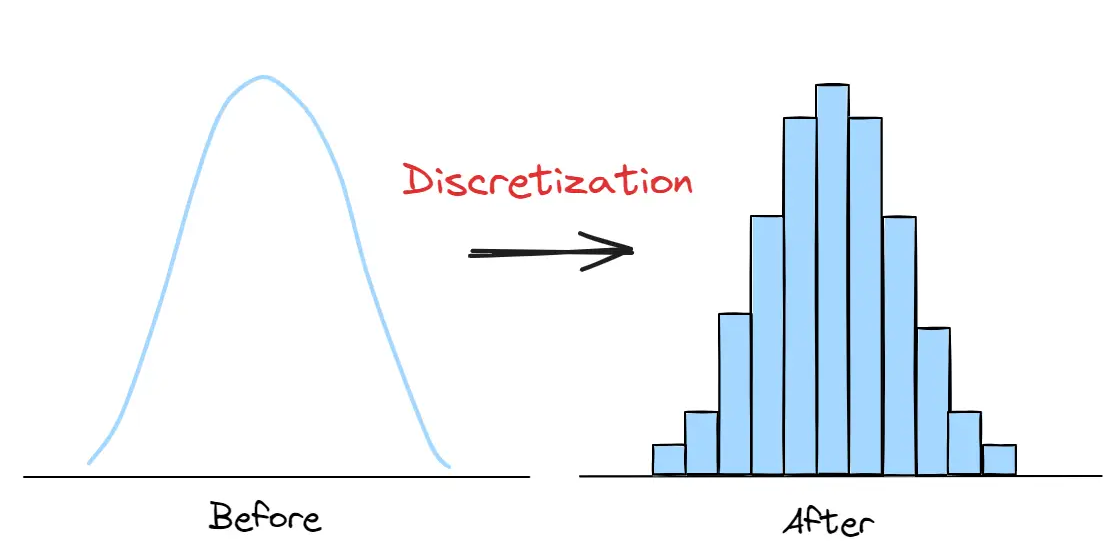
\includegraphics[width=5.20833in,height=\textheight,keepaspectratio]{../../images/discretizacao.png}
\end{center}
\end{frame}

\begin{frame}{Discretização de dados}
\phantomsection\label{discretizauxe7uxe3o-de-dados-1}
Técnicas comuns de discretização:

\pause

\begin{itemize}
\tightlist
\item
  \textbf{Discretização equi-probabilística:} Essa técnica envolve a
  divisão dos dados em intervalos de tamanho igual, de modo que cada
  intervalo contenha aproximadamente a mesma quantidade de observações.
\end{itemize}

\pause

\begin{itemize}
\tightlist
\item
  \textbf{Discretização equi-distante:} Nessa técnica, os dados são
  divididos em intervalos de tamanho igual, com base em uma distância
  predefinida.
\end{itemize}
\end{frame}

\begin{frame}{Discretização de dados}
\phantomsection\label{discretizauxe7uxe3o-de-dados-2}
\begin{itemize}
\tightlist
\item
  \textbf{Discretização por quartis:} Os dados são divididos em quartis,
  com base nos valores de corte que dividem os dados em quatro partes
  iguais.
\end{itemize}

\pause

\begin{itemize}
\tightlist
\item
  \textbf{Discretização por frequência:} Os dados são divididos em
  intervalos com base na frequência de observações em cada intervalo.
\end{itemize}
\end{frame}

\begin{frame}{Discretização de dados}
\phantomsection\label{discretizauxe7uxe3o-de-dados-3}
\begin{itemize}
\tightlist
\item
  \textbf{Binarização:} A binarização é uma técnica de transformação de
  dados que converte valores quantitativos em valores binários (0 ou 1)
  com base em um valor de corte.
\end{itemize}

\begin{columns}[T]
\begin{column}{0.5\linewidth}
\begin{center}
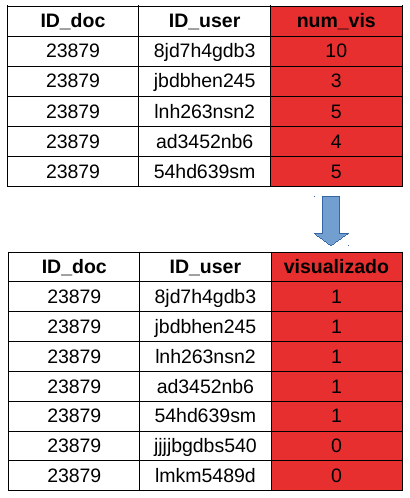
\includegraphics[width=5.20833in,height=\textheight,keepaspectratio]{../../images/fig05.png}
\end{center}
\end{column}

\begin{column}{0.5\linewidth}
\begin{center}
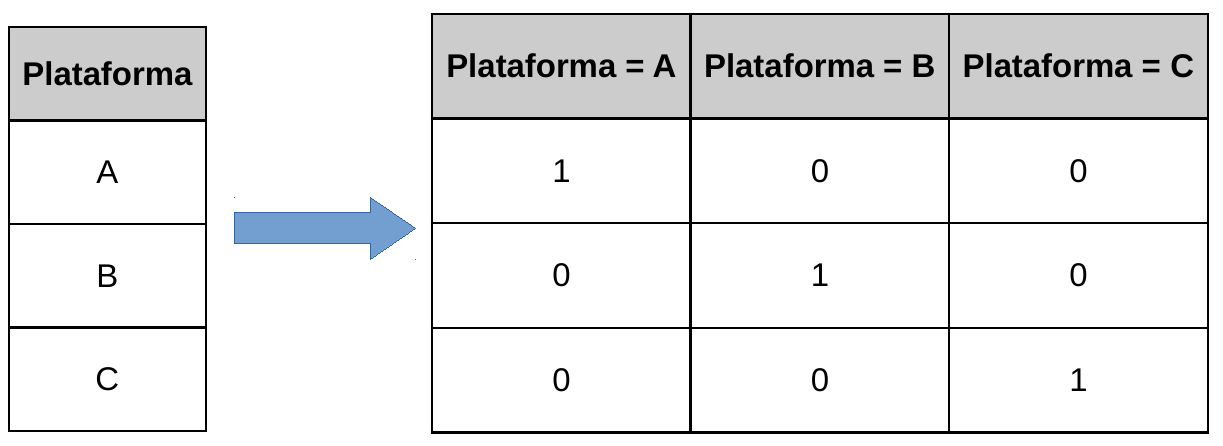
\includegraphics[width=10.41667in,height=\textheight,keepaspectratio]{../../images/fig08.png}
\end{center}
\end{column}
\end{columns}
\end{frame}

\begin{frame}{References}
\phantomsection\label{references}
\phantomsection\label{refs}
\begin{CSLReferences}{1}{0}
\bibitem[\citeproctext]{ref-madow1983incomplete}
Madow, W. G., H. Nisselson, I. Olkin, D. B. Rubin, National Research
Council (U.S.). Panel on Incomplete Data, Assembly of Behavioral, and
Social Sciences (U.S.). Panel on Incomplete Data. 1983. \emph{Incomplete
Data in Sample Surveys: Theory and Bibliographies}. Incomplete Data in
Sample Surveys. Academic Press.

\end{CSLReferences}
\end{frame}




\end{document}
